%\documentclass[10pt,twocolumn,twoside]{IEEEtran}
%\documentclass[journal]{IEEEtran}
\documentclass[journal]{new-aiaa}
%\documentclass[conf]{new-aiaa} for conference papers
\usepackage[utf8]{inputenc}
% The following packages can be found on http:\\www.ctan.org
\usepackage{graphics} % for pdf, bitmapped graphics files
\usepackage{epsfig} % for postscript graphics files
\usepackage{mathptmx} % assumes new font selection scheme installed
\usepackage{times} % assumes new font selection scheme installed
\usepackage{amsmath} % assumes amsmath package installed
\usepackage{amssymb}  % assumes amsmath package installed
\usepackage{algorithm}
% \usepackage[utf8]{inputenc}
\usepackage[noend]{algpseudocode}
\usepackage{graphicx}
\usepackage[font=small,labelfont=bf]{caption}
\usepackage{epsfig}
\usepackage{ulem}
\usepackage{verbatim}
\usepackage{amsfonts}
\usepackage{mathrsfs}
\usepackage{breqn}
\usepackage{xcolor}
\usepackage{mathtools}
\usepackage{caption}
\usepackage{subcaption}
%\usepackage[numbers]{natbib}
%\usepackage{varwidth}
%\usepackage{resizegather}
%\usepackage{euler}
\DeclarePairedDelimiter{\ceil}{\lceil}{\rceil}
\newcommand{\qd}{\hfill{\qed}}
\def\ba{\begin{array}}
\def\ea{\end{array}}
\newcommand{\beq}{\begin{equation}}
\newcommand{\eeq}{\end{equation}}
\newcommand{\bq}{\begin{eqnarray}}
\newcommand{\eq}{\end{eqnarray}}
\newcommand{\bqn}{\begin{eqnarray*}}
\newcommand{\eqn}{\end{eqnarray*}}
\newcommand{\bee}{\begin{enumerate}}
\newcommand{\eee}{\end{enumerate}}



\RequirePackage{ifthen}
\usepackage{amssymb,mathrsfs,wasysym}
%\usepackage{amsthm}
\usepackage{tikz}
\usepackage{url}
\usetikzlibrary{shadows}
\usetikzlibrary{shapes}

\newcommand{\always}{\square}
\newcommand{\eventually}{\Diamond}
\renewcommand{\next}{\ocircle}
\newcommand{\until}{\hspace{1mm}\mathcal{U}\hspace{1mm}}
\newcommand{\untilc}{\mathcal{U}}
\newcommand{\release}{\hspace{1mm}\mathcal{R}\hspace{1mm}}
\newcommand{\true}{\relax\ifmmode \mathit{True} \else \em True \/\fi}
\newcommand{\false}{\relax\ifmmode \mathit{False} \else \em False \/\fi}
\newcommand{\aand}{\hspace{1mm}\wedge\hspace{1mm}}
\newcommand{\oor}{\hspace{1mm}\vee\hspace{1mm}}
\newcommand{\set}[1]{\left\{#1\right\}}
\newcommand{\norm}[1]{\left\lVert#1\right\rVert}
\newtheorem{theorem}{Theorem}
\newtheorem{definition}{Definition}
\newtheorem{rem}{Remark}
\newtheorem{note}{Note}
% correct bad hyphenation here
% \hyphenation{op-tical net-works semi-conduc-tor}

\setlength{\textfloatsep}{10pt plus 1.0pt minus 2.0pt}
\begin{document}

\title{Receding Horizon Synthesis and Dynamic Allocation of UAVs to Fight Fires}

\author{Joshua~Shaffer,~
	Estefany~Carrillo,~
	and~Huan~Xu, Member, IEEE%\vspace*{-7mm}% <-this % stops a space
	\thanks{J. Shaffer, E. Carrillo, and H. Xu are with the Department of Aerospace Engineering,
		University of Maryland, College Park,
		MD 20740, USA. e-mail: \{jshaffe9, ecarril2\} @terpmail.umd.edu, mumu@umd.edu.}
	\thanks{This work was partially funded by Lockheed Martin.}}% <-this % stops a space


% As a general rule, do not put math, special symbols or citations
% in the abstract or keywords.

\maketitle



% As a general rule, do not put math, special symbols or citations
% in the abstract or keywords.
\begin{abstract}
This paper explores the design of a high-level mission planner and controller for managing UAVs fighting a wildfire through the utilization of reactive synthesis and dynamic allocation of the UAVs as resources to the fires. Reactive synthesis provides a formal means of guaranteeing the UAVs transition to areas of fire, refill on water, and land as defined by LTL specifications. Dynamic allocation coordinates the behavior of multiple UAVs through assignments to regions of fire based on a cost function that takes into effect the fire locations, distance to the domain edge, and other UAV locations. Modifications to a standardized horizon template guarantee that the inclusion of static obstacles in the scenario still maintains the overall realizability of the formal specifications in the receding horizon framework. For six fire scenarios, this paper shows the effectiveness of multiple UAV fleets in slowing down the progression of fires from reaching the domain edge. Lastly, our results and successful application expand discussion on the utilization of reactive synthesis in larger task spaces and the implications of abstracting UAV transitions for use in formal methods.
\end{abstract}

% Note that keywords are not normally used for peerreview papers.
%\begin{IEEEkeywords}
%Controller synthesis, Allocation processes, Receding Horizon control, Linear Temporal Logic.
%\end{IEEEkeywords}


% For peer review papers, you can put extra information on the cover
% page as needed:
% \ifCLASSOPTIONpeerreview
% \begin{center} \bfseries EDICS Category: 3-BBND \end{center}
% \fi
%
% For peerreview papers, this IEEEtran command inserts a page break and
% creates the second title. It will be ignored for other modes.
%\IEEEpeerreviewmaketitle

\section{Introduction}
% The very first letter is a 2 line initial drop letter followed
% by the rest of the first word in caps.
% 
% form to use if the first word consists of a single letter:
% \IEEEPARstart{A}{demo} file is ....
% 
% form to use if you need the single drop letter followed by
% normal text (unknown if ever used by the IEEE):
% \IEEEPARstart{A}{}demo file is ....
% 
% Some journals put the first two words in caps:
% \IEEEPARstart{T}{his demo} file is ....
% 
% Here we have the typical use of a "T" for an initial drop letter
% and "HIS" in caps to complete the first word.

The economic burden of wildfires on the United States (in 2016 \$US) exceeds \$63.5 billion annually due to damages, and more than \$7.6 billion is spent annually to fight said fires \cite{c0}. Current methods of fighting fires involve numerous man hours and piloted vehicles, including aerial vehicles capable of dropping large amounts of suppressant over regions of fire. Aerial vehicles with suppression capabilities have served as critical tools in slowing down the growth of fires due to their far greater range of maneuverability when compared to ground crews \cite{c21}. Often these aircraft can change the outcome of a wildfire if used to attack a small fire early enough. As discussed in \cite{c1}, unmanned aerial vehicles (UAVs) pose a huge benefit to traditional firefighting methods, with the foremost advantage of creating additional ``eyes in the sky" and supply drops. These uses of UAVs have motivated numerous agencies to explore such options in the last decade. In terms of direct suppression, though, automated UAVs were used to extinguish fires on their own as was mechanically demonstrated on a small, single-UAV scale in \cite{c2}. The creation of a fleet of autonomous drones for quick response to fledging small-scale wildfires, in turn, could limit the number of required personale to a site and produce more efficient results. For the purposes of research in UAV autonomy, a design problem such as this allows for the exploration and further assessment of multiple methods in automation.

One such method, reactive synthesis, provides a means for generating correct-by-construction controllers for complex systems. Synthesized controllers take into account system and environment variables with varying dynamics, progress and safety specifications, and initial conditions. The primary benefit of this method is the correct-by-construction attribute: the realized controller will satisfy the specifications designed by the user as long as the environment behaves according to the assumptions made. Programmers are not required to ``handcraft" individual behaviors of a system under specific conditions (of which are often error prone) and can instead focus on defining the system and specifications. The major pitfall of reactive synthesis is the computational complexity in dealing with dynamic environments as discussed in \cite{c10}.

Despite such disadvantages, the implementation of reactive synthesis is suitable when considering finite abstractions of systems with small state spaces. Without this type of framework, most problems become infeasible to handle only with reactive synthesis. For example, consider a scenario involving the path planning of a robot that must always avoid any number of arbitrarily placed obstacles on a 10x10 grid. The synthesized controller must account for every possible obstacle location ($2^{100}$ permutations), resulting in an inordinate amount of computation time. Unfortunately, real problems can easily involve this scenario's scale of permutations in the environment, hence the restrictions enforced on reactive synthesis. 

When the high-level design of a system does involve this scale of environmental permutations and state space, solutions typically seek to discretize the synthesis problem or approach the problem from a different perspective. Discretization appears in the use of receding horizon control in \cite{c3} and the use of decentralized controllers for multiple agents in \cite{c4}. Both examples break down the top-level synthesis problem into smaller, discrete pieces for the computation benefits. On the other hand, \cite{c5} approached their synthesis problem with a focus on resolving deadlock under specific environment conditions instead of directly avoiding dynamic obstacles. In each of the presented cases, the problem description focuses on a limited task space and how the solution can handle larger sets of actions from an environment. In \cite{c3}, \cite{c4}, and \cite{c5}, the task space encompasses up to 4 progress statements for each scenario. 
%Even with the problem space discretized, both examples presented rely on other methods to achieve the desired results. In [CITE],... and in [CITE]... Clearly a gap still exists between designing the high-level controllers for robust autonomous systems that reside within reality and utilizing reactive synthesis to fully realize such designs. In truth, attempting to close the gap presents a futile challenge, one that .... 

For the purposes of fighting large, dynamic fires with a single autonomous UAV, a high-level controller created with just reactive synthesis would quickly present an impractical solution if the design should accommodate a fairly granular state space with a large number of tasks. Further expanding this concept to a whole fleet of UAVs, the problem becomes worse due to an increase in the number of system variables. Even with decentralized controllers for each UAV, more system variables would need to be introduced to describe coordination and behaviors between the decentralized UAV controllers. To alleviate the computational complexity on reactive synthesis in this regard, the coordination of UAVs can be handled by a dynamic allocation process. %As discussed, the more arbitrary the scenario is (preferred given the idea that a single design should fit for most applications), the more likely that a design based solely on reactive synthesis would become impractical due to increased permutations in environmental variables. \textcolor{red}{REVISE SOME}%As discussed later on in this paper (in the \textit{Implementation} section), breaking down the synthesis problem still provided excessive state spaces to explore, and the futility of attempting a singular synthesized solution became readily apparent.

Dynamic allocation presents an autonomous method for assigning resources in an ever-changing environment. Recent approaches include clustering techniques and formulating the allocation problem in the form of a multi-objective problem. In \cite{c14}, a partitioning-based task allocation strategy is proposed to decide on the assignment of agents in dynamic disaster environments by applying the K-means clustering algorithm. In \cite{c15} and \cite{16}, the resource allocation problem is framed as a multi-objective optimization problem of minimizing the extinguishing time and resource utilization cost, solved by the use of evolutionary algorithms in \cite{c15} and by mathematical programming techniques in \cite{16}. 

We propose an allocation strategy to address the assignments of UAVs for our fire fighting scenario. If the fleet of UAVs are treated as resources to manage with respect to a changing fire landscape, dynamic allocation would serve well in assigning the UAVs to specific fires. Assignments would depend upon factors in the behavior of the fires such as density, intensity, ability to spread, and more. Perhaps readily apparent, though, is that an allocation algorithm would not necessarily be constructed to control the UAVs within the state space defined, nor would the algorithm manage other high-level system aspects associated with the UAVs, such as suppressant control and decisions on emergency landings. Building these high-level behaviors into an allocation algorithm requires ``handcrafting" these behaviors for all scenarios, an approach that synthesis, on the other hand, is well suited to avoid.

To integrate the two discussed methods, reactive synthesis and dynamic allocation, we utilize the receding horizon framework for reactive synthesis as discussed in \cite{c10}. As far as we have found, \cite{c6} first touched upon the idea of manipulating the receding horizon framework for decomposing the synthesized problem and decentralizing the planning procedure. For their purposes, this idea resulted in the ability of multiple agents to satisfy high-level specifications through only considering other agents that entered their local horizon. For our purposes, decentralizing the planning procedure allows for dynamic allocation to arrange the order of progress goals specified in the synthesized controller in real-time. Through this, we seek to reconcile the strengths and weaknesses of the two discussed methods to create a high-level mission planner and controller for implementation in a fire fighting scenario. 

%This paper is motivated by the concept of combining reactive synthesis with other methods to work in tandem and provide a solution to a high-level problem with a large number of tasks to achieve. We seek to build upon the work described above by exploring a multi-agent system in a complex dynamic environment while meeting a task-space on an order of magnitude greater than the aforementioned task spaces. 

The rest of the paper follows as such. In \textit{Section II}, we present subjects pertinent to the exploration of our topic, primarily in relation to reactive synthesis. In \textit{Section III}, we present the fire fighting scenario, including environment and system definitions. \textit{Section IV} discusses our proposed solution, followed by the implementation of our solution in \textit{Section V}. In \textit{Section VI}, we present the outcomes to our tested cases, followed by our conclusions in \textit{Section VII}.

\section{Preliminaries}

Linear temporal logic (LTL) is utilized for describing specifications within the reactive synthesis framework. LTL makes use of boolean system variables that serve as atomic propositions (AP), and LTL formulas are built through APs with logic connections and temporal modal operators. Logic connections include $\lnot$ (negation), $\lor$ (or), $\land$ (and),  and $\implies$ (implication). Temporal modal operators include $\next$ (next), $\always$ (always), $\eventually$ (eventually), and $\until$ (until). LTL formulas that only utilize logic connections are referred to with $\varphi$. Through the use of LTL, a broad range of specifications can be written to describe the behaviors of a system (or environment). We point the reader to the preliminaries section of \cite{c7} for an expanded description of LTL as it pertains to our purposes.

Reactive synthesis provides a method for generating controllers within the context of a defined environment and system as specified through LTL. One of the most commonly used forms for these LTL formulas is general reactivity(1) (GR(1)), the assume-guarantee form shown in Eq. (\ref{GR1}),
\begin{equation}
\label{GR1}
\begin{aligned}
(\varphi_{init}^{e} \land \bigwedge_{i \in I_r} \always \varphi_{s,i}^{e} \land \bigwedge_{i \in I_f} \always \eventually \varphi_{p,i}^{e}) \longrightarrow \\ (\varphi_{init}^{s} \land \bigwedge_{i \in I_s} \always \varphi_{s,i}^{s} \land \bigwedge_{i \in I_g} \always \eventually \varphi_{p,i}^{s}).
\end{aligned}
\end{equation}
From the above equation, the propositional formula $\varphi_{init}$  describes the initial condition of the environment or system (denoted by superscript $e$ or $s$, respectively), $\varphi_{s,i}$  describes safety specifications, and $\varphi_{p,i}$ describes progress specifications. \cite{c7} proved that when the system and environment specifications are written in the framework shown in Eq. (\ref{GR1}), the synthesis of a system controller that fulfills the specifications while subject to the environment will occur in polynomial time. The proof of such, though, provides no guarantee that the polynomial time required will fall within a practical time-limit, due to the formulation's limiting dependency on the total amount of permutations between the system and environmental states.

\begin{figure}
	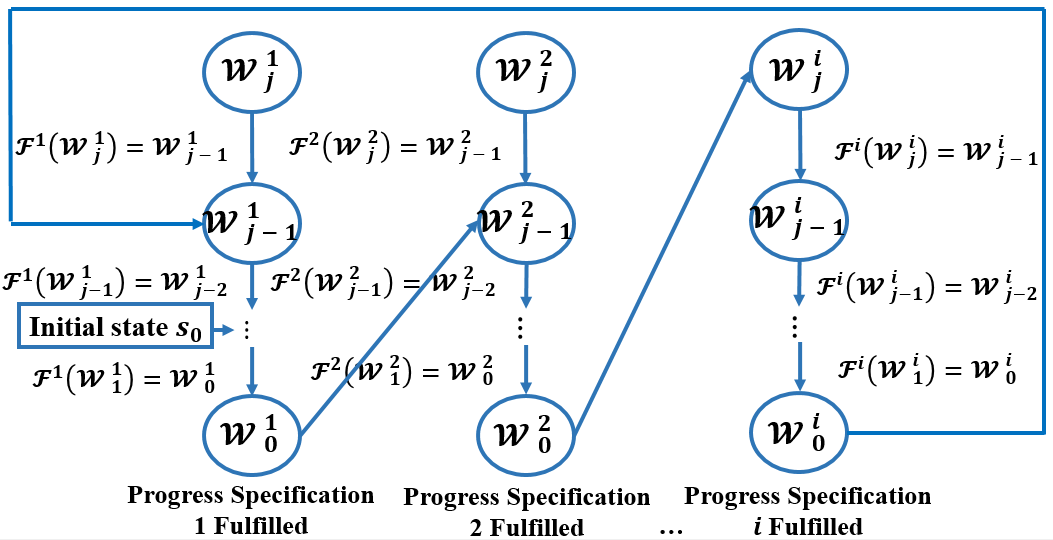
\includegraphics[width = 1 \linewidth]{RHFramework}
	\centering
	\caption{Segmentation of state space and example of ordered set flow-down performed in receding horizon framework, as described in \cite{c10}.}
	\label{RhFrame}
	\vspace*{-2mm}
\end{figure}

\cite{c8}, \cite{c9}, and \cite{c10} have explored reactive synthesis within a receding horizon (RH) framework. The primary benefit of utilizing RH is the segmentation of the state space for both the environment and system into separate horizons. Each horizon provides a smaller problem to synthesize a controller for, and the combination of these controllers form a single controller that obeys the specifications written for the total system and environment. The primary disadvantage of RH is that while each horizon itself can be optimized, the total sum is not. Other sources have explored methods of optimizing control with respect to time-based rewards on each horizon, such as in \cite{c9}, but such optimization is forgone in this paper. 

Implementation of RH revolves around, for each progress specification, segmenting the total system state space into regions $\mathcal{W}_j^i$ so that, when placed into properly constructed ordered sets represented by $\mathcal{F}^i(\mathcal{W}_j^i)$, the system variables will converge to meeting each progress statement for the system, i.e. $\mathcal{W}_0^i$. Here, $i$ represents the system progress statement $i \in I_g$, and $j$ indexes the ordered regions $\mathscr{W}$ about the progress specification $i$. This process is displayed in Fig. \ref{RhFrame}. Following the basis laid out by \cite{c10}, each region consists of its own GR(1) specification (shown in Eq. (\ref{RH})), constructed so that the synthesized controller will move the system states towards the next region within the ordered set (eventually leading to $j = 0$) and fulfill the top level GR(1) specification,

\begin{equation}
\label{RH}
\begin{aligned}
\Psi_{j}^{i} = ((s \in \mathcal{W}_j^i) \land \Phi \land \bigwedge_{i \in I_r} \always \varphi_{s,i}^{e} \land \bigwedge_{i \in I_f} \always \eventually \varphi_{p,i}^{e}) \longrightarrow \\
(\bigwedge_{i \in I_s} \always \varphi_{s,i}^{s} \land \always \eventually(s \in \mathcal{F}^i(\mathcal{W}_j^i)) \land \always \Phi).
\end{aligned}
\end{equation}

In Eq. (\ref{RH}), $s$ refers to the system state. The formula $\Phi$ consists of all limitations on the states of system, preventing the system from making transitions to or initializing within states that are not allowed. This tautology prevents individual synthesized controllers from creating transitions to states that are infeasible for longer horizons.

\section{Problem Formulation}
The high-level problem scenario this paper explores is presented as such. A 450-by-450 meter region of flat grassland, segmented by various large-scale obstacles, is experiencing a wildfire. Fires spread from starting regions under fixed environmental conditions, and the starting fire locations are arbitrary. A base of operations exists near the edge of the region and contains a fleet of $N$ UAVs for fighting the fire. Fig. \ref{probpartition} visualizes the abstracted region for this problem. 

 \begin{figure}
	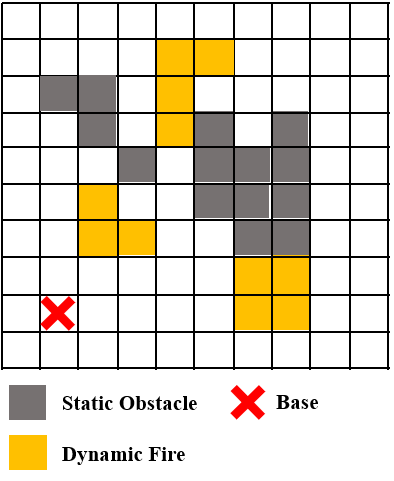
\includegraphics[width = 0.6 \linewidth]{GridPartitionVert}
	\centering
	\caption{2D grid partition of problem location with environmental indicators}
	\label{probpartition}
%	\vspace*{-3mm}
\end{figure}

Each UAV holds a varying level of suppressant for dumping on the fire, from High (100\%), Medium (66\%), Low (33\%), to Empty (0\%), associated with a total water volume of $W_v = $ 125 liters. Each individual UAV contains a radio for communicating with base, GPS for determining position, and any other sensors required for lower-level controllers. Each UAV's average flight speed, $v$, is approximately $15$ m/s. Design constraints on the UAVs require the need for periodic landing and enforcement of in-flight kinematics resembling fixed-wing behavior. The design goal of this fleet is to significantly slow down the fires' spread to the outer edge of the domain as compared to the fires' natural growth.

The formal definition of the abstracted system space is provided in Definition \ref{system}.

\begin{definition}
	\label{system}
	The state set is defined as $S = S_p \times S_o \times W$, where the position set is $S_p = \{(1, 1), (1, 2), (2, 1),... (10, 10)\}$, the orientation set is $S_o = \{0^\circ, 90^\circ, 180^\circ, 270^\circ\}$, and the water level set is $W= \{0\%,33\%, 66\%, 100\%\}$. A single UAV at any given time is represented as an element $s \in S$. For the elements of $s$, $s_{x,y}$ is used to represent the position tuple (where $x$ and $y$ can take the position values of the tuple), $s_o$ is used to represent the orientation, and $w$ is used to represent the water level.
\end{definition}

Note that the above definition implies that each position represents a cell of 45-by-45 meters. Furthermore, viable transitions for the UAVs between elements in the state space are defined assuming 3 transition scenarios, a sped up counterclockwise turn, a sped up clockwise turn, and a straight drive ahead. These transition scenarios result in the following transition system described in Definition \ref{definition7}, visualized in Fig. \ref{transitions}.

\begin{definition}
	\label{definition7}
	The transition relation for the state set $S$ is defined as $T = \{s \to s' \in R \subseteq S \times S\}$, where elements $s \to s' \in R$ are defined for each allowable $s'$ per $s \in S$ under the following conditions.
	
	If $s_o = 0^\circ$: 
	
	-Option 1: $s'_{x,y} = (s_x+1,$ $s_y)$ with $s'_o = 0^\circ$
	
	-Option 2: $s'_{x,y} = (s_x+1,$ $s_y+1)$ with $s'_o = 90^\circ$
	
	-Option 3: $s'_{x,y} = (s_x+1,$ $s_y-1)$ with $s'_o = 270^\circ$
	
	If $s_o = \pi/2^\circ$: 
	
	-Option 1: $s'_{x,y} = (s_x,$ $s_y+1)$ with $s'_o = 90^\circ$
	
	-Option 2: $s'_{x,y} = (s_x+1,$ $s_y+1)$ with $s'_o = 0^\circ$
	
	-Option 3: $s'_{x,y} = (s_x-1,$ $s_y+1)$ with $s'_o = 180^\circ$
	
	If $s_o = \pi^\circ$: 

	-Option 1: $s'_{x,y} = (s_x-1,$ $s_y)$ with $s'_o = 180^\circ$

	-Option 2: $s'_{x,y} = (s_x-1,$ $s_y+1)$ with $s'_o = 90^\circ$

	-Option 3: $s'_{x,y} = (s_x-1,$ $s_y-1)$ with $s'_o = 270^\circ$
	
	If $s_o = 3\pi/2^\circ$: 

	-Option 1: $s'_{x,y} = (s_x,$ $s_y-1)$ with $s'_o =270^\circ$

	-Option 2: $s'_{x,y} = (s_x-1,$ $s_y-1)$ with $s'_o = 180^\circ$

	-Option 3: $s'_{x,y} = (s_x+1,$ $s_y-1)$ with $s'_o = 0^\circ$
\end{definition}

 \begin{figure}
	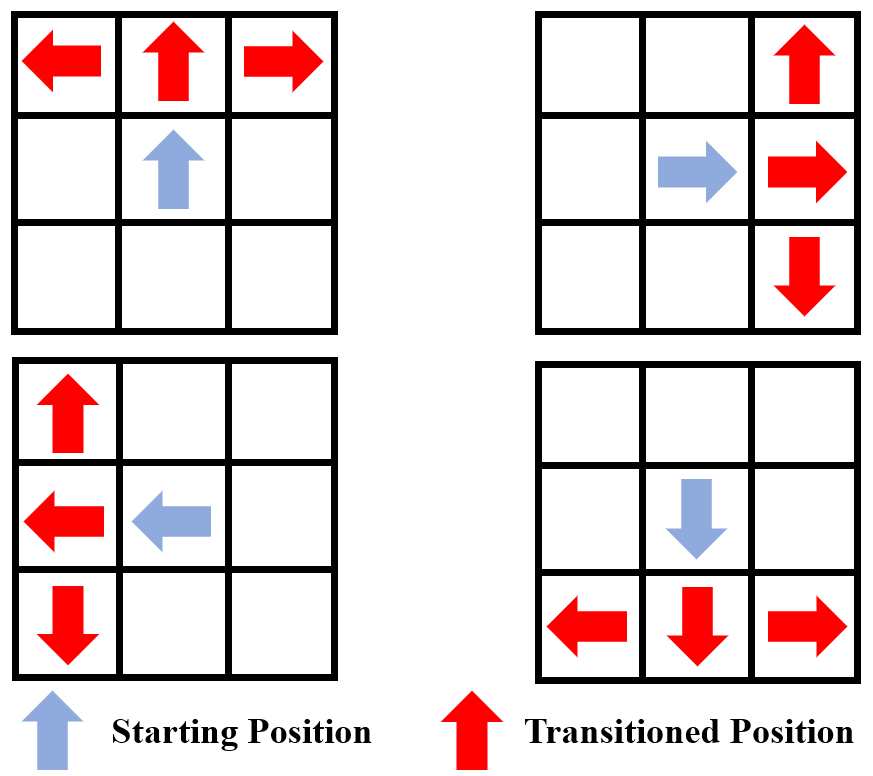
\includegraphics[width = 0.6 \linewidth]{Transitions}
	\centering
	\caption{Possible transitions for UAV within grid given starting orientation and location}
	\label{transitions}
%	\vspace*{-3mm}
\end{figure}

Depending on the location of static obstacles and boundaries, elements within the described transition relation are restricted from the general case if they violate the \textit{reachability} property of the system, as defined through Definition \ref{reachable}. This implies that the existence of obstacles requires limitation on allowable states $S$ in the system specifications. A graph search for paths that lead to dead ends is an accessible way of determining these states.

\begin{definition}
	\label{reachable}
	The system $S$ is defined as \textit{reachable} if there exists a path of states, composed of a finite number of subsequent transitions in $s \to s' \in T \subseteq S \times S$, such that all $s \in S$ can be eventually reached from any other initial state $s \in S$.
\end{definition}

The formal definition of the abstracted environment space is provided in Definition \ref{env}. Note that this general environment definition is expansive in size (up to $2^{100+N}$ combinations). Also note that this environment definition serves as an abstraction to a more complicated fire growth model, described in further detail in the \textit{Implementation} section.

\begin{definition}
	\label{env}
	The fire environment is defined as $F_{x,y} = (x, y) \times \{True, False\}$ for any valid choice of $x$ and $y$ in the system domain, excluding the base location. The element $f_{x,y} \in F_{x,y}$ corresponds to the presence of fire (i.e. $True$ or $False$) associated with the tuple $(x,y)$. The total possible environment is the combination of all $F_{x,y}$ sets with the landing signal sets of each UAV, i.e. $E = F_{1,1} \times F_{1,2} \times F_{2,1}, \times ... F_{10,10} \times S_{land,1} \times S_{land,2} \times... S_{land,N}$, where $S_{land, n} = \{True, False\}$ corresponds to the landing signal of the $n^{th}$ UAV.
\end{definition}

Under these formal definitions on the system and environment, the desired design for each UAV are as follows. [LTL specifications shown provide formal context to the intention of the written specifications]. First, each UAV must fly to any region in the state space associated with an active fire (Eq. \ref{goal_specs}), dumping a fraction of its water supply if possible (Eq. \ref{goal_specs_watdump}). 

\begin{equation}
\begin{aligned}
\bigwedge_{(x',y')} \always (f_{x',y'} \longrightarrow \eventually (s_{x,y} \leftrightarrow (x', y')))
\end{aligned}
\label{goal_specs}
\end{equation}

\begin{equation}
\begin{aligned}
\bigwedge_{(x',y')} \always ((w > 0\% \land f_{x',y'} \land (s_{x,y} \leftrightarrow (x', y'))) \\ \leftrightarrow \next w = w - 33 \%)
\end{aligned}
\label{goal_specs_watdump}
\end{equation}

 Next, each UAV must return to base for replenishing water supplies when empty (Eq. \ref{watspecs}) and the water level must refill to the max level when the UAV reaches base (Eq. \ref{watspecs2}). Note that $base$ is an AP that is $True$ when $s_p$ matches the associated $(x,y)$ tuple for the base.
 
 \begin{equation}
 \begin{aligned}
\always (w = 0\% \longrightarrow \eventually base) 
 \end{aligned}
 \label{watspecs}
 \end{equation}
 
  \begin{equation}
 \begin{aligned}
 \always ((w = 0\% \land base) \leftrightarrow \next w = 100\%)
 \end{aligned}
 \label{watspecs2}
 \end{equation}

 The UAVs may experience landing signals and must land for prolonged periods of time in the next available region not consumed by fire (Eq. \ref{stopreq}). 
 
  \begin{equation}
 \begin{aligned}
 \always ((s_{land,n} \land \lnot f_{x,y}) \longrightarrow (\next s_{x,y} \leftrightarrow s_{x,y}))
 \end{aligned}
 \label{stopreq}
 \end{equation}
 
 Lastly, the order in which fires are addressed must be prioritized by their capability of reaching the domain edge, and UAVs must allocate themselves in a manner that increases their combined effect on the environment. This specification is an open area of design, one in which a formal specification describing the priority queue of active fires would require further environment and system definitions. \textcolor{red}{Don't think this is a smooth transition to the next section...}
% \begin{figure}
%	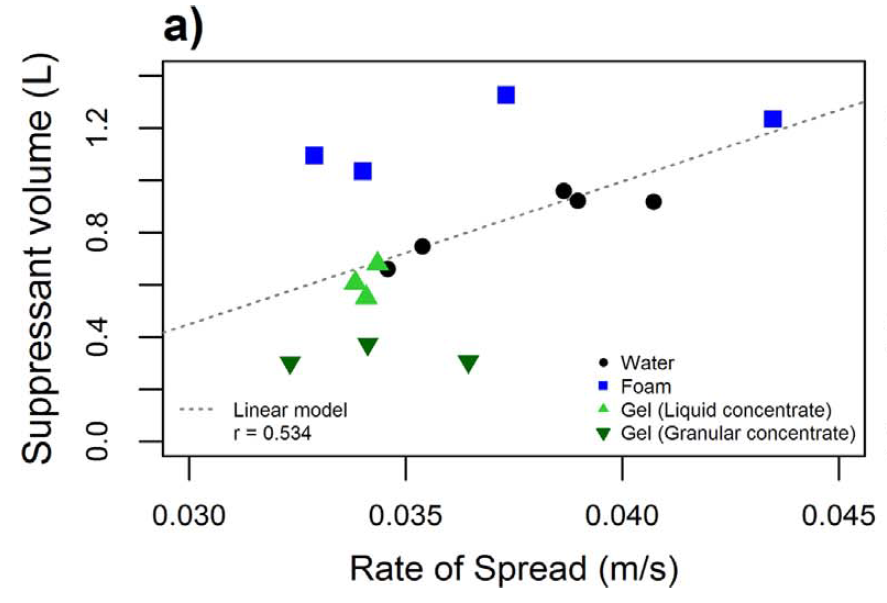
\includegraphics[width = 1.0 \linewidth]{FireRateCITE}
%	\centering
%	\caption{Tested suppressant volumes required for extinguishing fires per spread rates in 1.5 x 3 meter test area, pulled directly from \cite{c11}}
%	\label{FireRateSpread}
%	\vspace*{-3mm}
%\end{figure}

%\begin{table*}[t]
%	\centering
%	\caption{Fire growth behavior}
%	\label{table_1}
%	\scalebox{1}{
%		\begin{tabular}{|c||c||c||c||c|}
%			\hline
%			\multicolumn{1}{|p{3cm}|}{\centering Fire intensity level} & \multicolumn{1}{|p{3cm}|}{\centering Fire spread rate $f_r$ (m/s)} & \multicolumn{1}{|p{3cm}|}{\centering Required suppressant volume per square meter $v_r$ (L/m\textsuperscript{2})} & \multicolumn{1}{|p{3cm}|}{\centering Time before fire spreads $t_f$ (s)} & \multicolumn{1}{|p{3cm}|}{\centering Fuel consumption at intensity increase $f_c$} \\ 
%			\hline
%			Low & 0.035 & 0.156 & 1287 & 1 \\ 
%			\hline
%			Medium & 0.040 & 0.211 & 1125 & 2 \\
%			\hline
%			High & 0.045 & 0.267 & 999 & 3 \\
%			\hline
%		\end{tabular}
%	}
%\vspace*{-3mm}
%\end{table*}

%\textcolor{red}{()}. This equation, while not determined directly by a physical law, is created to capture an effectiveness of coordination in UAVs, a desired behavior of the UAVs detailed later on. The equation shows that each time a combined amount of water is dropped, the amount registered as effective to the fire scales around a nominal amount of 40\% of the total tank amount $W_v$.

%As mentioned before, the design goal for this problem scenario is to create a high-level autonomous controller to dictate the overall behavior of the fleet for tackling any generic fire situation while maintaining the desired design specifications per UAV. For a given fire scenario, we seek to determine the required minimum number of UAVs. Given any number of UAVs, success is achieved when the fleet can permanently extinguish all fires while maintaining a minimum level of total fuel.

%\vspace*{-3mm}
\section{Proposed Solution Method}
We propose a solution method to the formulated problem scenario that combines reactive synthesis with a dynamic allocation algorithm. These two methods form a high-level planner and controller that fulfills the design constraints imposed on each UAV and dictates the behavior of each one as well as their collective maneuvers. Fig. \ref{RHAlloc} depicts a conceptual view of the process of creating our solution and the duties that each method fulfills. Fig. \ref{AllocandGoal} depicts the direct relationship between the allocation process and a synthesized controller.

\begin{figure}
	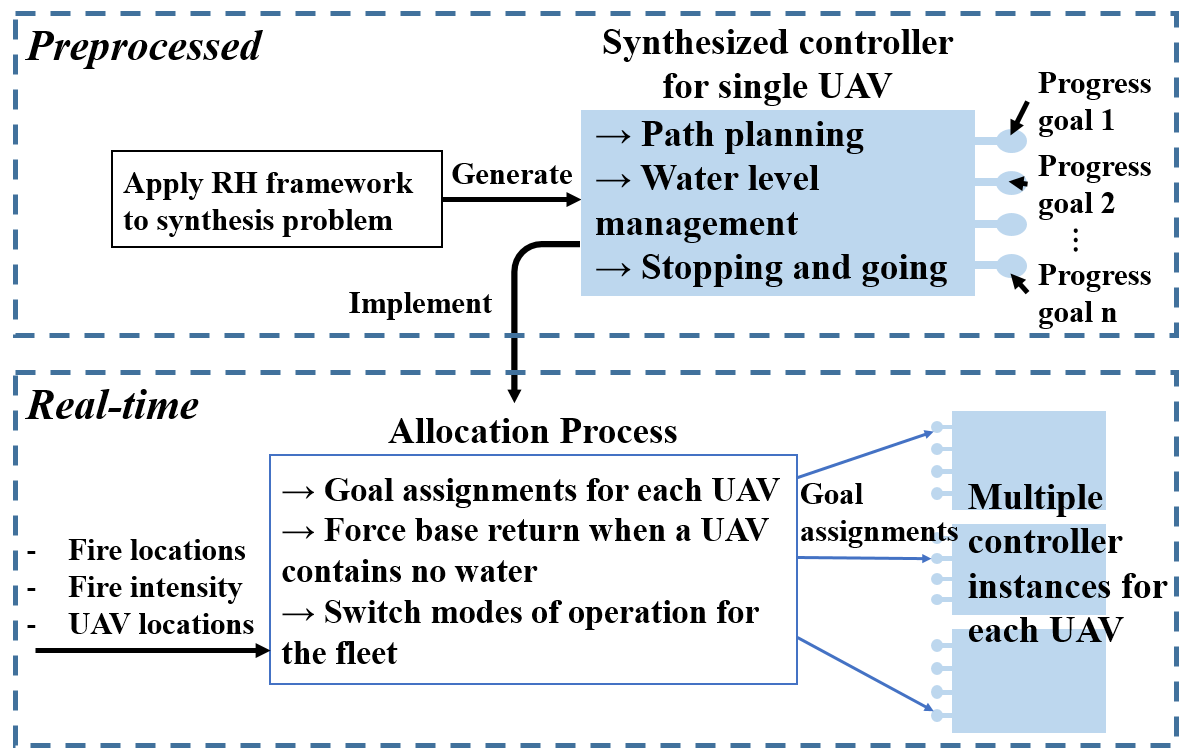
\includegraphics[width = 1.0 \linewidth]{SynthAlloc}
	\centering
	\caption{Diagram of creating the solution method and the responsibilities and roles for both the synthesized controllers and the allocation process during real-time implementation}
	\label{RHAlloc}
%	\vspace*{-3mm}
\end{figure}

 \begin{figure}
	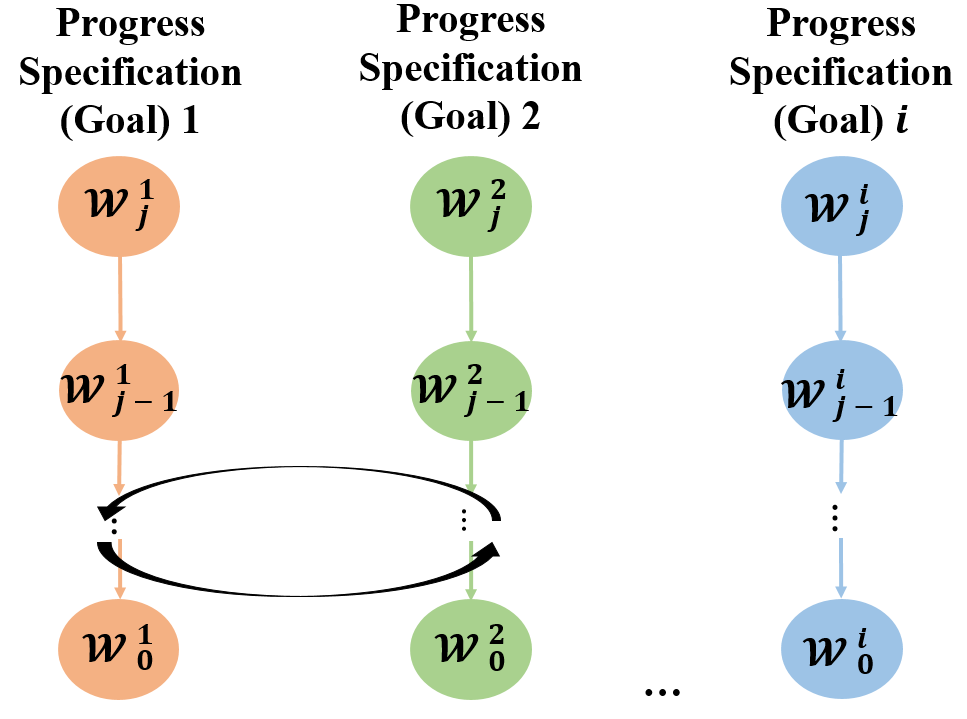
\includegraphics[width = 0.9 \linewidth]{AllocandGoals}
	\centering
	\caption{Diagram of allocation process rearranging the progress goal ordering (as depicted in Fig. \ref{RhFrame}) for a single UAV controller instance in real-time}
	\label{AllocandGoal}
%	\vspace*{-3mm}
\end{figure}

As shown in Fig \ref{RHAlloc}, a common synthesized controller is created for each of the UAVs through the RH framework with the duties presented. Given any arbitrary initial condition, the controller aims to progress to each viable partitioned space, these progress goals represented within Fig. \ref{RHAlloc} by the ``nodes" protruding from each rectangle. The order that the controller meets these progress statements for a single UAV, shown previously through the ordering of $\mathscr{W}^i$ in Fig. \ref{RhFrame}, is not dictated by the synthesized controller as typically performed within the RH framework. Instead, the allocation process decides which progress specification any single UAV should pursue, represented within Fig. \ref{AllocandGoal} by the switching of the ``nodes'" order for any given moment in time. Hence, the allocation process prioritizes and assigns which goals a single controller should meet next in real-time. The combination of these two methods in the described manner works to highlight the strengths of each method. The synthesized controllers manage various system oriented aspects of the design and path planning while allocation governs the fleet behavior through assignments of goals for each controller.

Previously mentioned in \cite{c2}, a physical scenario was constructed that dealt solely with one UAV gathering water, moving to another location, and dumping said water on the destination. \cite{c2} demonstrates the existence of lower level controllers that could manage the individual actions necessary to achieve the high-level planner and controller this paper proposes (at least for a smaller scale UAV). So, as often expressed in other sources dealing with high-level synthesized controllers, we assume there exists low-level controllers to dictate the motion of individual agents in real-time.

\begin{rem}
One caveat with regards to the solution explored in this paper is the, perhaps obvious, alternative solution. Suppose the design was created through a more ``handcrafted" approach, one without the uses of formal methods for verification. Utilization of a path planning algorithm (such as any of the on-line algorithms discussed in \cite{c18}) for sending UAVs to any given destination (i.e. a fire or base) from any starting condition, could be combined with the described top-level allocation process that managed the destinations for all UAVs together. A huge benefit of such an approach is that the dedicated path-planning algorithm could handle a greater variety of dynamic environments than a synthesized controller. However, the described approach could easily be susceptible to programming errors due to the necessity of creating the conditions that dictate other task-oriented operations of the UAV (such as those involving control of the water level, knowing when to land under what conditions, etc.), precisely the issue that reactive synthesis aims to resolve. This paper's proposed solution method seeks to explore and expand the capabilities of reactive synthesis as a formal method within a more granular environment and complex task space.
\end{rem}

%\vspace*{-3mm}
\section{Implementation}

This section describes the construction and operation of the synthesized controllers and allocation algorithm used for the high-level controller. Additionally, the simulation used to test such cases is also outlined.

%\vspace*{-3mm}
\subsection{Synthesis of Controllers in Receding Horizon framework}
The RH framework discussed requires individual synthesis problems about each progress goal while maintaining all safety specifications. For Eq. (\ref{goal_specs}) and (\ref{watspecs}), translated GR(1) goals involve always eventually driving the system to the regions holding fire or the base, invoked by the presence of fire or absence of held water. For creation of the actual specifications used in synthesis, we assume that the dynamic allocation process correctly interprets the required conditions which force the UAV to the base or fire (e.g. when the water level is empty, instead of the synthesized controller interpreting such and driving the UAV to base, the dynamic allocation recognizes and forces the UAV to prioritize the goal associated with base). As a result, Eq. (\ref{goal_specs}) and (\ref{watspecs}) are simply reinterpreted as Eq. (\ref{firegoal}) and (\ref{watgoal}), respectively. Therefore, the specifications used in synthesis will include the safety specifications shown in Eq. (\ref{goal_specs_watdump}), (\ref{watspecs2}), and (\ref{stopreq}) alongside these simplified goal specifications.

\begin{equation}
\begin{aligned}
\bigwedge_{(x',y')} \always \eventually (s_{x,y} \leftrightarrow (x', y'))
\end{aligned}
\label{firegoal}
\end{equation}

\begin{equation}
\begin{aligned}
\always \eventually base
\end{aligned}
\label{watgoal}
\end{equation}

For the common synthesized controller, the formal environmental description described beforehand is broken down to the relative signals as perceived by a single UAV and manipulated by either the allocation method or the naturally occurring environment. These Boolean variables consist of: $s_{land}$, representing whether or not the UAV needs to stop due to a landing signal; $f_d$, representing the presence of fire directly beneath the UAV; and $drop$, representing the allocation process's signal to a UAV for dropping water on the assigned goal location. Hence, the relative environment $E_r = \{s_{land}, f_d, drop\}$. 

The environment specifications for a single UAV are listed as follows: 

\begin{equation}
\varphi_{init}^{e} = \{\},
\label{EnvInit}
\end{equation}
\begin{equation}
\varphi_{s}^{e} = \{\},
\label{EnvSafety}
\end{equation}
\begin{equation}
\begin{aligned}
\varphi_{p}^{e} = \always \eventually drop \land \always \eventually \lnot s_{land} \land \always \eventually \lnot f_d,
\end{aligned}
\label{envprog}
\end{equation}

Eq. (\ref{EnvInit}) and (\ref{EnvSafety}) show that no guarantees are provided on the environment's initial condition and safety behavior, and (\ref{envprog}) states that always eventually allocation instructs the UAV to drop water, the UAV will experience engine failure, and the UAV will not be over fire.

The system consists of $S$ as described in Definition \ref{system}. Additional APs $goal$ and $base$ were created for when the UAV enters a specified goal location and the base location, respectively. These revised definitions are used to form updated specifications in GR(1) form for each set of horizons about each goal.

The system specifications from \textit{Section III} were formally defined about each goal tied to a tuple $(x,y)$ for each UAV :
\begin{equation}
\varphi_{init}^{s} = \Phi.
\label{UAVinit}
\end{equation}
Eq. (\ref{UAVinit}) reflects that a UAV will start in a state allowed by $\Phi$ (the RH tautology that governs feasible states). In this scenario, the tautology simply prevents the system from occupying any state that violates the conditions of Definition \ref{reachable} before the horizons have been applied.
\begin{equation}
\begin{aligned}
\varphi_{s,1}^{s} = \always ((s_{land} \land \lnot f_d) \leftrightarrow (\next s_{x,y} \leftrightarrow s_{x,y})),
\end{aligned}
\label{UAVStop}
\end{equation}
Eq. (\ref{UAVStop}) is the modified form of Eq (\ref{stopreq}), already in GR(1) form, replacing the global $f_{x,y}$ element with the local $f_d$ variable.

  \begin{equation}
\begin{aligned}
\varphi_{s,2}^{s} = \always (( w = 0 \%  \land goal \land base) \\ \leftrightarrow \next w = 100\%)
\end{aligned}
\label{waterlevmod}
\end{equation}

\begin{equation}
\begin{aligned}
\varphi_{s,3}^{s} = \always (( w > 0 \%  \land drop \land goal \land \lnot base) \\ \leftrightarrow \next w = w - 33 \%),
\end{aligned}
\label{UAVWaterLevel}
\end{equation}
Eq. (\ref{waterlevmod}) and Eq. (\ref{UAVWaterLevel}) are the modified versions of Eq. (\ref{goal_specs_watdump}) and Eq. (\ref{watspecs2}), respectively. In Eq. (\ref{waterlevmod}), the system reaching the base location has been replaced with the local $goal \land base$ proposition combination to enforce the notion that UAVs only fill up when reaching base if the base was also set as the goal.

\begin{equation}
\begin{aligned}
\varphi_{p}^{s} = \always \eventually goal,
\end{aligned}
\label{UAVProg}
\end{equation}
Lastly, Eq. (\ref{UAVProg}) is the generalized version of Eq. (\ref{firegoal}) and Eq. (\ref{watgoal}). Eq. (\ref{UAVProg}) models both since the allocation process is responsible for ensuring the conditions that drive the UAV to either the base location or a particular fire location, which serve as the current goal.

% \begin{figure}
%	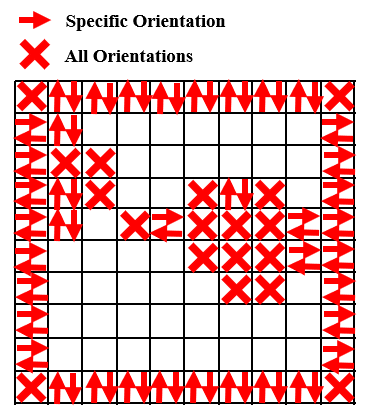
\includegraphics[width = 0.5 \linewidth]{Phi}
%	\centering
%	\caption{All positions and orientations not included in $\Phi$}
%	\label{Phi}
%\end{figure}

\begin{figure}
	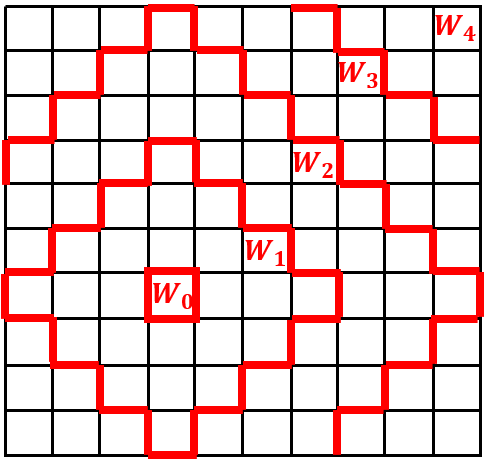
\includegraphics[width = 0.5 \linewidth]{WPartitionPic}
	\centering
	\caption{RH partitions for progress statement centered on position (4,4)}
	\label{WPart}
%	\vspace*{-3mm}
\end{figure}

Eq. (\ref{UAVinit}) - (\ref{UAVProg}) along with the environment definitions form Eq. (\ref{totalsynth}), the synthesis problem about each progress goal. This formulation captures the intended behavior of the original specifications while enabling the allocation method to dictate which goals are prioritized in which order. 

\begin{equation}
\label{totalsynth}
\begin{aligned}
\Psi^{x',y'} = \varphi^e_{init} \land \varphi^e_s \land \varphi^e_p \longrightarrow \\ \varphi^s_{init} \land \varphi^s_{s,1} \land \varphi^s_{s,2} \land \varphi^s_{s,3} \land \varphi^s_p \land \always \Phi
\end{aligned}
\end{equation}

To apply the RH framework, the state space must be segmented into horizons $\mathcal{W}_j^{x',y'}$ about every possible goal region. A formal definition for such is provided by Definition \ref{definition6}, and Fig. \ref{WPart} visualizes such for a single goal by allocation.

\begin{definition}
	\label{definition6}
	Horizons are defined as $\mathcal{W}^{x',y'}_j = \{s \in S$ $|$ $3(j-1)\le$ $|s_x - x'| + |s_y - y'|$ $ \le 3j$ where $j > 0\}$. $\mathcal{W}^{x',y'}_0$ refers to $goal$.
\end{definition}

These horizons are utilized to form the individual $\Psi^{x',y'}_j$ specifications used in the RH framework. This formal definition is easy to apply to this problem since it requires a simple calculation while automating the synthesis process. Unfortunately, these horizons do not account for static obstacle placement creating the restrictions represented by $\Phi$, and blind application will create unrealizable specifications. To circumvent such, a horizon modification algorithm is applied during synthesis to maintain the realizability of all RH specifications, shown in Algorithm \ref{alg:Wgen}.

\begin{algorithm}
	\caption{$\mathcal{W}^{x',y'}_j$ Modification during Synthesis}\label{alg:Wgen}
	\begin{algorithmic}[1]
		\Procedure{Synthesis$\_$Goal}{$x',y'$}\Comment{Synthesis controllers from all initial conditions for the $x',y'$ goal location}
		\For{$0 \le j \le N$}
		\For{$s \in \mathcal{W}_j^{x',y'}$}
		\State Synthesize controller given $x',y'$ goal and current $s$
		\If{Controller == None}
		\State Remove $s$ from $\mathcal{W}_j^{x',y'}$
		\State Add $s$ to $\mathcal{W}_{j+1}^{x',y'}$
		\EndIf
		\EndFor
		\EndFor
		\EndProcedure
	\end{algorithmic}
\end{algorithm}	

\subsubsection{Receding Horizon Modification and Proof of Specification Validity}

\begin{theorem}
	Given a modified version of the system in Definition \ref{system} which has removed some accessible states and transitions through the addition of static obstacles but still maintains the \textit{reachability} property described in Definition \ref{reachable}, and by using the initial horizons $\mathcal{W}^{x',y'}_j$ described in Definition \ref{definition6} applied with the horizon modification algorithm described by Algorithm \ref{alg:Wgen}, the specification for each horizon surrounding each progress goal, $\Psi_{j}^{x',y'}$, will remain realizable, preserving the RH framework guarantees on the overall specification.
\end{theorem}

%\begin{proof}
	First, we maintain that the overall specification (Eq. (\ref{totalsynth})) is realizable for the modified system description given no horizons and any allowable initial condition. Because of such, a horizon-based synthesized solution exists that fulfills the framework and definitions provided in \cite{c10}. 
	
	%Given the receding horizon template pictured in Fig. \ref{WPart} and formally described in Definition \ref{definition6}, guarantees regarding the satisfaction of our overall specification through the RH framework can be provided under modified horizon definitions.
	
	%First, we only consider a subset of the total state definition that includes only location and orientation. This %is directly allowed for all horizons since specifications regarding the water levels require the position and %orientation states to reach desired goal locations $g_{i,p}$ (including the base of operations). This subset is %defined as $S_{sub} = s_p \times s_o$. We assume that a further subset of $S_{sub}$ exists (coined $S_{s}$) %such that, when combined with the transition relation defined by Definition \ref{definition7} having $S$ %replaced by $S_s$, the total state set and transition relation holds path-connectedness as defined by %Definition \ref{definition3}.
	
	Given the Definition \ref{definition6} description of the receding horizons $\mathcal{W}^{x',y'}_j$ for any individual goal $(x',y')$, reachability (Definition \ref{reachable}) implies that for any state sequence $\pi$ that starts and leads from $s \in \mathcal{W}^{x',y'}_j$ to a state $s_f$ with $s_{f,x,y} = (x',y')$, said sequence $\pi$ must contain at least one $s \in \mathcal{W}^{x',y'}_k$ for all $0 < k \le j$. Under the modified system definition, all available $\pi$ sequences for some $s \in \mathcal{W}^{x',y'}_j$ may also need to include $s \in \mathcal{W}^{x',y'}_r$ for some $r > j$, i.e. the only available path to the goal may require the state to move into horizons away from the goal before moving back through horizons towards the goal due to the presence of obstacles. The presence of such a sequence that includes paths with $s \in \mathcal{W}^{x',y'}_{r > j}$ as the only valid path immediately violates the conditions for the receding horizon specification $\Psi_{j}^{x',y'}$. To address this violation, modifications to the horizons, as shown in Algorithm \ref{alg:Wgen}, are made during synthesis to maintain the condition that a path $\pi$ does not contain any $s \in \mathcal{W}^{x',y'}_{r > j}$.			
	
	As controllers are synthesized around each goal and for each initial condition $s_i$ within each set $\mathcal{W}^{x',y'}_j$, starting with $j = 0$ and incrementing, realizability failures are direct results of the lack of a system path to the horizon $\mathcal{W}^{x',y'}_{j-1}$ that remains only in $\mathcal{W}^{x',y'}_{j}$. This is a result of the failure to satisfy $\Psi_{j}^{x',y'}$ since the overall specification $\Psi^{x',y'}$ is realizable. Because a path starting at the initial condition $s_i$ that fulfills the global specification must exist on the global scale and none of the sets $\mathcal{W}^{x',y'}_j$ overlap per index $(x',y')$, the path must enter into $\mathcal{W}^{x',y'}_{j+1}$ due to the reachability property stated before. Through the algorithm, this state $s_i$ is removed from $\mathcal{W}^{x',y'}_{j}$ and added to $\mathcal{W}^{x',y'}_{j+1}$. All intermediate states between the initial condition and horizon $\mathcal{W}^{x',y'}_{j+1}$ are also moved to the next horizon since each state is tested as an initial condition in Algorithm \ref{alg:Wgen}, and these states cannot serve as viable initial conditions themselves. Therefore, the revised $\mathcal{W}^{x',y'}_{j+1}$ contains the original set $\mathcal{W}^{x',y'}_{j+1}$ plus all states from $\mathcal{W}^{x',y'}_{j}$ that could not serve as initial conditions to reach the next horizon of $\mathcal{W}^{x',y'}_{j-1}$ (or goal if $j-1 = 0$). This statement serves as a recursive assignment for each horizon $j$, shifting states back horizons until a new horizon set for a goal is defined such that each $s \in \mathcal{W}^{x',y'}_{j}$ starts a path $\pi$ contained solely in $\mathcal{W}^{x',y'}_{j}$ that reaches $\mathcal{W}^{x',y'}_{j-1}$. Because of this, $\Psi_{j}^{x',y'}$ is realizable for all goals, all horizons, and all initial conditions, maintaining the guarantees provided by the RH framework used from \cite{c10}.
%\end{proof}

The benefit of the approach used by Algorithm \ref{alg:Wgen} is that the viability test for an initial condition is made during synthesis and construction of controllers, saving on computation time since the horizons are not evaluated and modified before synthesis. Hence the original horizon definition serves as a starting point that may or may not be preserved for each goal and is only modified when necessary.

%\vspace*{-4mm}
\subsection{Dynamic allocation}

In this paper, we propose an efficient method for managing the dynamic allocation of UAVs to fire perimeter locations that spread with time. The allocation process considers four main parameters: wind direction; proximity of the UAVs to fire locations; proximity of fires to the domain boundary; and the amount of burn-through time provided by any suppressant acting on the fire. We assume that the fire model (which determines the previous parameters and is explained further in the \textit{Simulation} subsection) and it's corresponding perimeter is correctly abstracted into the cells used by the synthesis process (i.e. any cell that contains the fire perimeter is interpreted as holding fire and is made available for allocation).

The allocation process is ran by assigning each UAV to an unassigned fire that minimizes a cost function relative to the UAV. This cost is calculated as the weighted sum of: the distance between the fire and the UAV; the fire's distance from the boundary edge; the alignment of the fire's direction alongside the wind; and the amount of suppressant acting on the fire. We refer to this cost fuction as $g$ as shown in Eq. (\ref{AllocEqn}).
\begin{equation}
\label{AllocEqn}
\begin{aligned}
\min_{f\in F} g(f,x) = d_{f}*\norm{x-f} + \\ e_f*\min(\norm{edge - f}_{x_{min}, y_{min}, x_{max}, y_{max}}) - \\ w_f*wind_{speed}*(x \cdot [\sin(wind_{azimuth}), \cos(wind_{azimuth})])+\\ b_f*suppressant\_time\_left(f),
\end{aligned}
\end{equation}
where $d_{f}$ is used as penalty weight for the distance between UAV location $x$ and fire $f$ $\in$ $F$ ($F$ represents the set of all fire locations). This first term in Eq. (\ref{AllocEqn}) seeks to drive UAVs towards their closest fires. The coefficient $e_f$ represents a penalty weight on fires that are further from the outer edge of the domain, and $w_f$ is an importance weight on fires further along the direction of the wind. These two terms drive UAVs towards fires that are closer to the domain edge and further along the direction of the wind as compared to the origin. Finally, coefficient $b_{f}$ corresponds to a penalty on the remaining time for suppressant already present at the fire. This penalizes UAVs for repeatedly dropping suppressant on fires that just recently had suppressant added.

These weights represent ``knobs" for heuristically tuning the allocation of UAVs to individual fires. Ideally, we aim to have the UAVs prioritize fire perimeters that are moving along the wind direction and approaching the edges of the domain foremost. The distance from fire and burn-through time terms act to ``spread out" the allocation of UAVs when the wind and edge terms are less severe. Through initial testing, we achieved the desired behaviors using the evaluated terms and standard units by choosing the coefficients $d_f$, $e_f$, $w_f$, and $b_f$ as 0.1, 1.0, 0.1, and 0.02, respectively.

%\vspace*{-4mm}
\subsection{Simulation}

To implement the solution and test its ability to meet the problem scenario, the synthesized controllers and allocation algorithm were constructed in Python alongside a simplified fire simulation following the wavelet differential equations and the Rothermel spread equation provided in FARSITE \cite{FARSITE}. FARSITE models the fire fronts as propagating wavelets, with the fire spread rate calculated by the Rothermel spread equation serving as the main indication of intensity. \cite{rosthermel} provides the valuation of the Rothermel spread equation for various fuel types and climates, shown in Fig. \ref{fire_rates}. For the simulation, we assumed the fuel type was SH7, which is shrubbery in a dry climate, and approximated the spread rates for 3 levels of wind speed. Table \ref{table_23} provides these approximations for each wind speed. At each update time for the fire, the calculated spread rate of a fire vertex along the perimeter was also adjusted with a +/-10\% deviation to provide further variation in the fire front growth across each simulation. Additionally, the fire front model's perimeter was abstracted into distinct fire regions for use by the dynamic allocation process. 

\begin{figure}
	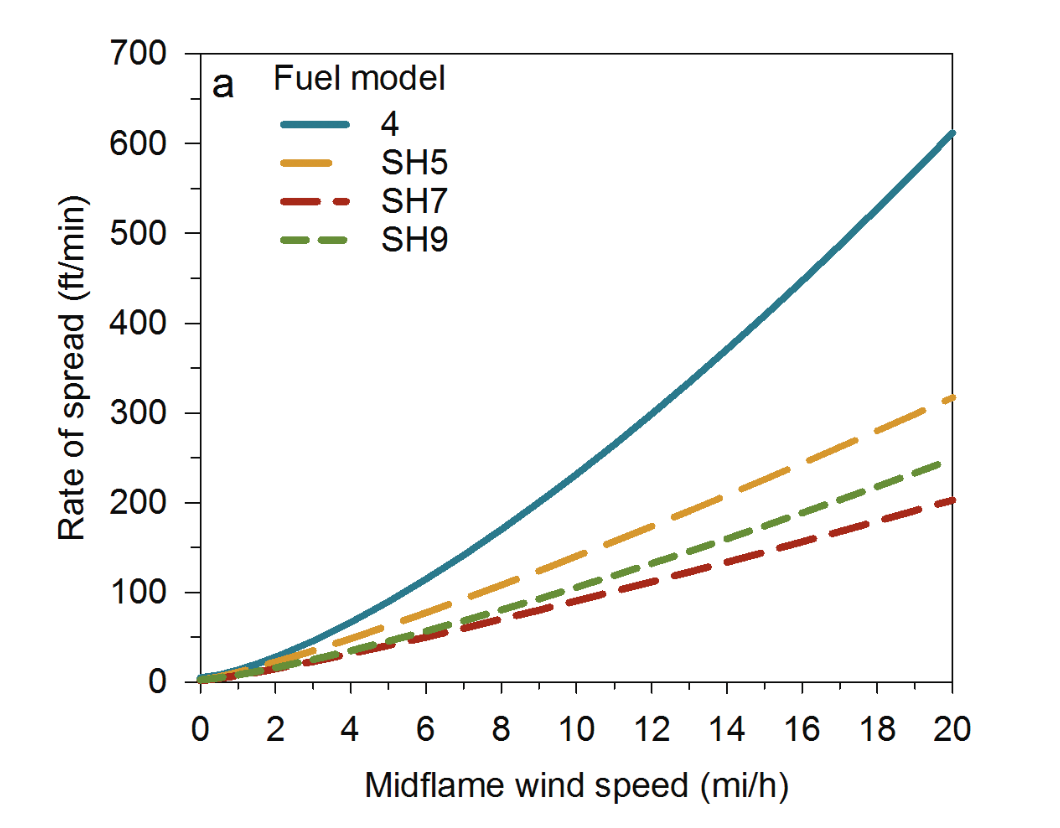
\includegraphics[width = 1 \linewidth]{fire_rates}
	\centering
	\caption{Fire spread rates for various fuel models, pulled directly from \cite{rosthermel}}
	\label{fire_rates}
	%	\vspace*{-3mm}
\end{figure}

\begin{table}[H]
	\centering
	\caption{Simulation wind speeds and corresponding spread rates}
	\label{table_23}
	\scalebox{0.8}{
		\begin{tabular}{|c||c|}
			\hline
			\multicolumn{1}{|p{2.5cm}|}{\centering Wind Speed \\ (m/s)} & \multicolumn{1}{|p{2.5cm}|}{\centering Rate of Spread \\ (m/min)} \\ 
			\hline
			1.0 (Low) & 3.0 \\ 
			\hline
			4.0 (Medium) & 18.0 \\
			\hline
			8.0 (High) & 48.0 \\
			\hline
		\end{tabular}
	}
\end{table}

Fire suppression mechanics are a relatively unknown area of research, and simulations typically assume that obstacles (both static and dropped suppressant) simply stop or greatly slow the spread rate at that specific location on a fire front, either indefinitely for static obstacles or a limited time for suppressant (referred to as the burn-through time). The placement of temporary obstacles in our simulation provided the direct mechanisms in which the fire was slowed down at any point by a UAV. The dropping of suppressant was modeled after the line length and burn-through times for 1500 liters of suppressant, as discussed in \cite{australiafirereport}. For a 1500 liter suppressant drop across 45 meters, the burn-through time is approximately 2 hours. We assumed that a linear relationship exists between the amount of suppressant and the burn-through time, i.e. 125 liters constitute about 10 minutes of burn-through, and each fractional drop of 125 liters on an area added the same proportional amount of 10 minutes to the current burn-through time. Additionally, we assumed a linear relationship between the rate of growth of a fire vertex within a suppressant area and the burn-through time left. The endpoints on this linear relationship were 0\% of normal growth rate for full burn-through time left and 5\% of normal growth for no burn-through time left. This relationship was included to add conservative stress the UAVs' ability to suppress the fires. Lastly, the geometry associated with suppressant drops was ignored, i.e. any suppressant dropped on the fire front was assumed to align itself so as to correctly block the fire within that region. 

The UAVs were modeled to follow simplified kinematics and assumed to still maintain the transitions described in the problem description at each time step. Additionally, the UAVs were assumed to require 4 minutes anytime they were forced to stop, either by a random stop signal or stopping at the base to pick up suppressant.

\begin{figure}
	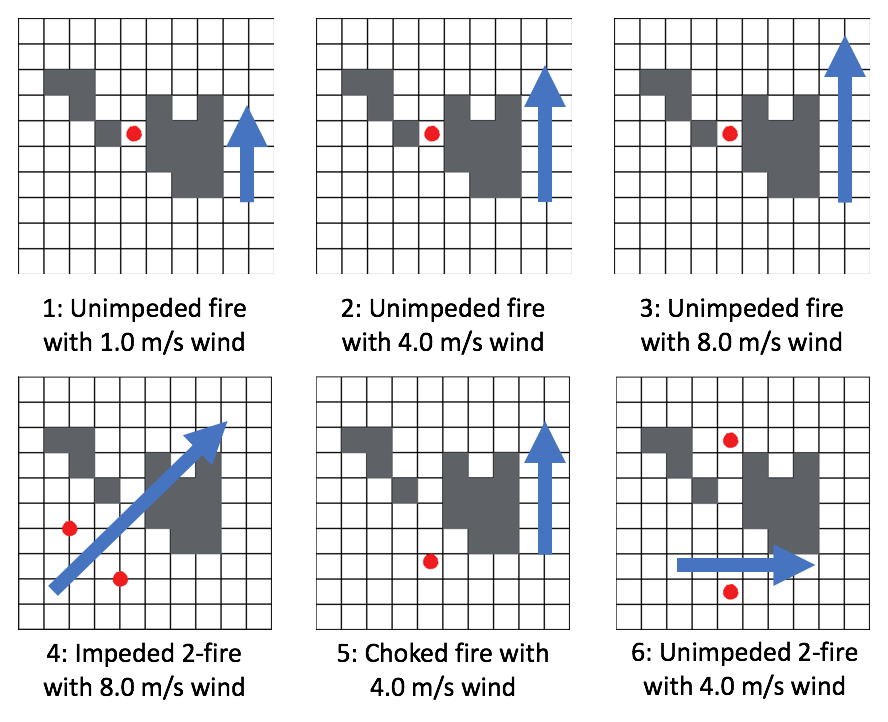
\includegraphics[width = 1 \linewidth]{scenario_overview}
	\centering
	\caption{Fire scenario visualizations, initial fire-placement and wind conditions}
	\label{scenarioFire}
%	\vspace*{-3mm}
\end{figure}

Various fire scenarios' initial conditions and parameter settings were constructed for the purposes of testing the controllers. These fire scenarios were aimed at testing the capabilities of the UAVs to slow down all fires from reaching the borders and gauge the effectiveness of different fleet numbers. These scenarios are provided in Fig. \ref{scenarioFire}. The simulation cycled through multiple iterations on each scenario, testing the effectiveness of up to 4 fleet members. The average time for the fire to reach the outer edge on each scenario and fleet number combination was calculated. For all scenarios, the UAVs started at the base location.

%\vspace*{-3mm}
\section{Results}

TuLiP \cite{c12} was utilized to realize and synthesize the controllers associated with each region $\mathcal{W}_j^{x',y'}$. On an Intel i5-6500 CPU @ 3.20 GHz processor, this total process, approximately 250 regions $\mathcal{W}$, took on the order of 8 hours. In addition to the large amount of time to synthesize all of the individual controllers, numerous memory issues came up throughout the process, even with a system limit of 16 GB of RAM. The total size of the synthesized controllers was approximately 2 GB.

For each scenario tested, simulations where conducted 100 times to assess the fleet of UAVs' ability to slow down the spread of the fire to the domain edges, provided each UAV experiences a 1\% chance of a random stop signal for every transition time (3 seconds in all scenarios). The results were compiled and displayed in box and whisker plots shown in Fig. \ref{fig:test}, \ref{fig:test2}, and \ref{fig:test3}. 

\begin{figure}
	\centering
	\begin{subfigure}{.25\textwidth}
		\centering
		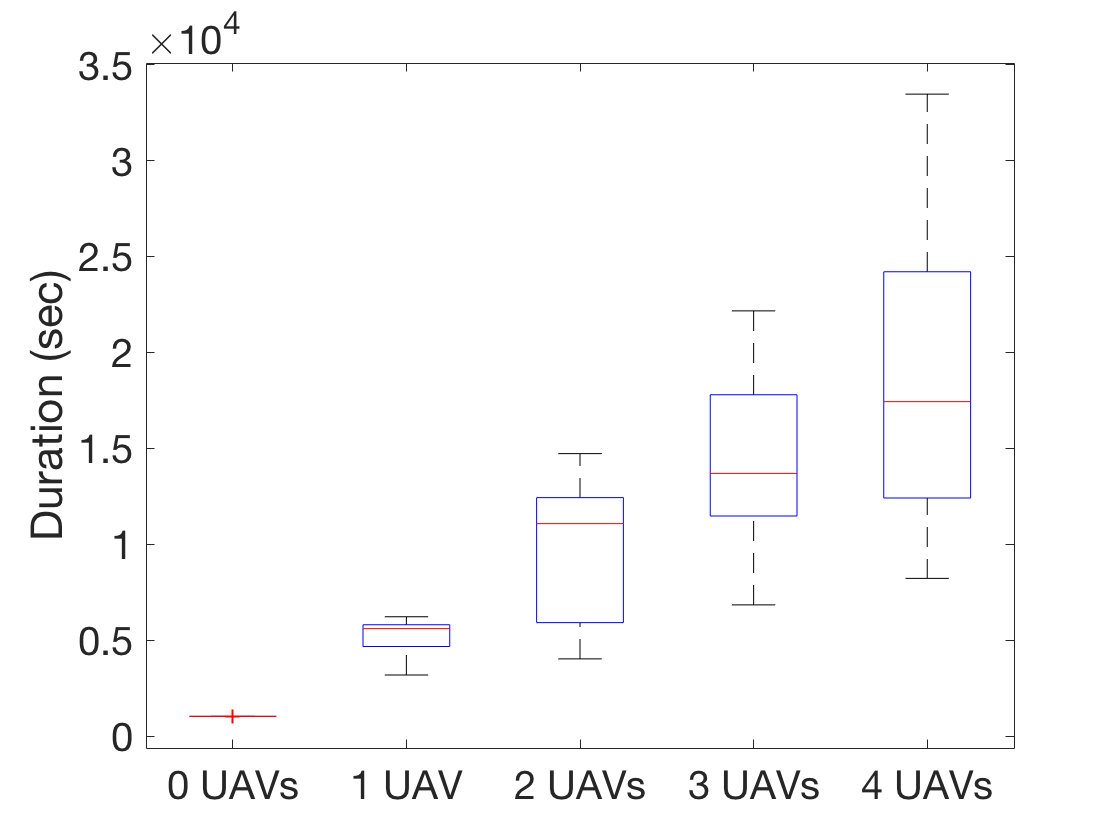
\includegraphics[width=1\linewidth]{case1_resultsgraph}
		\caption{Scenario 1}%: Mid-start with low north wind}
		\label{fig:sub1}
	\end{subfigure}%
	\begin{subfigure}{.25\textwidth}
		\centering
		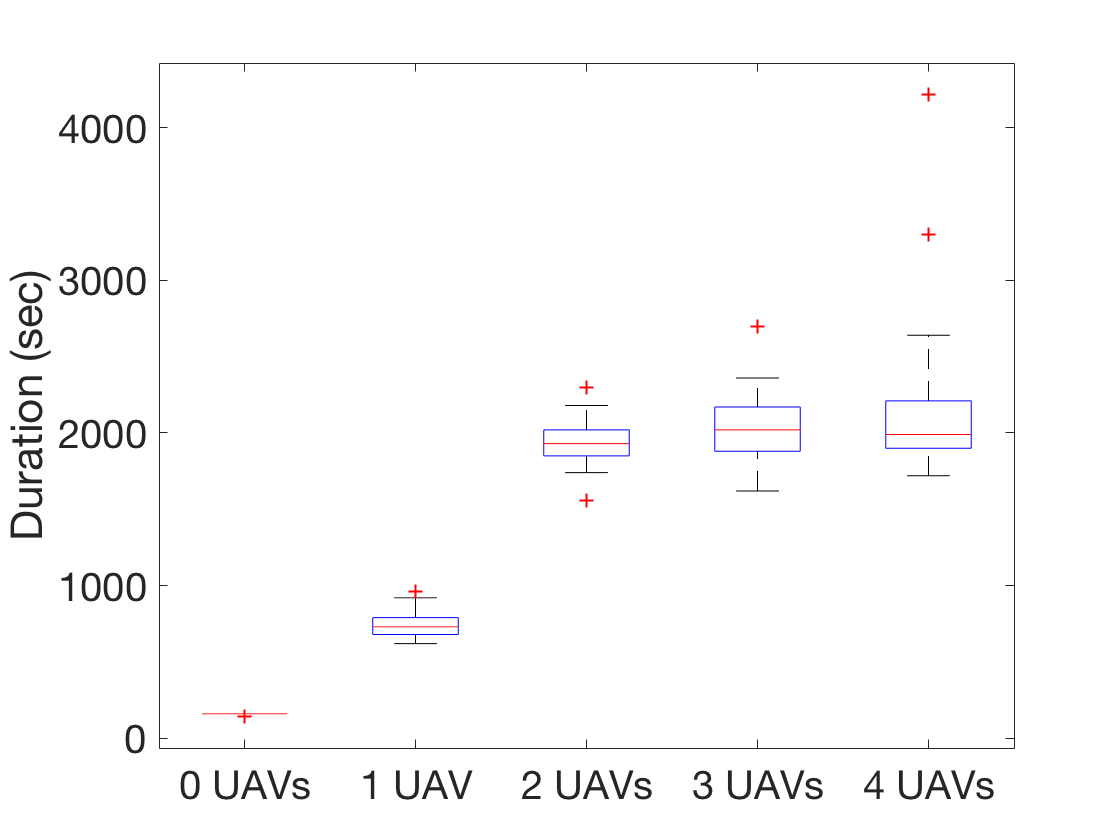
\includegraphics[width=1\linewidth]{case2_resultsgraph}
		\caption{Scenario 2}%: Mid-start with medium north wind}
		\label{fig:sub2}
	\end{subfigure}
	\caption{Distributions of simulation results for scenario 1 and scenario 2}
	\label{fig:test}
	\vspace*{-2mm}
\end{figure}

\begin{figure}
	\centering
	\begin{subfigure}{.25\textwidth}
		\centering
		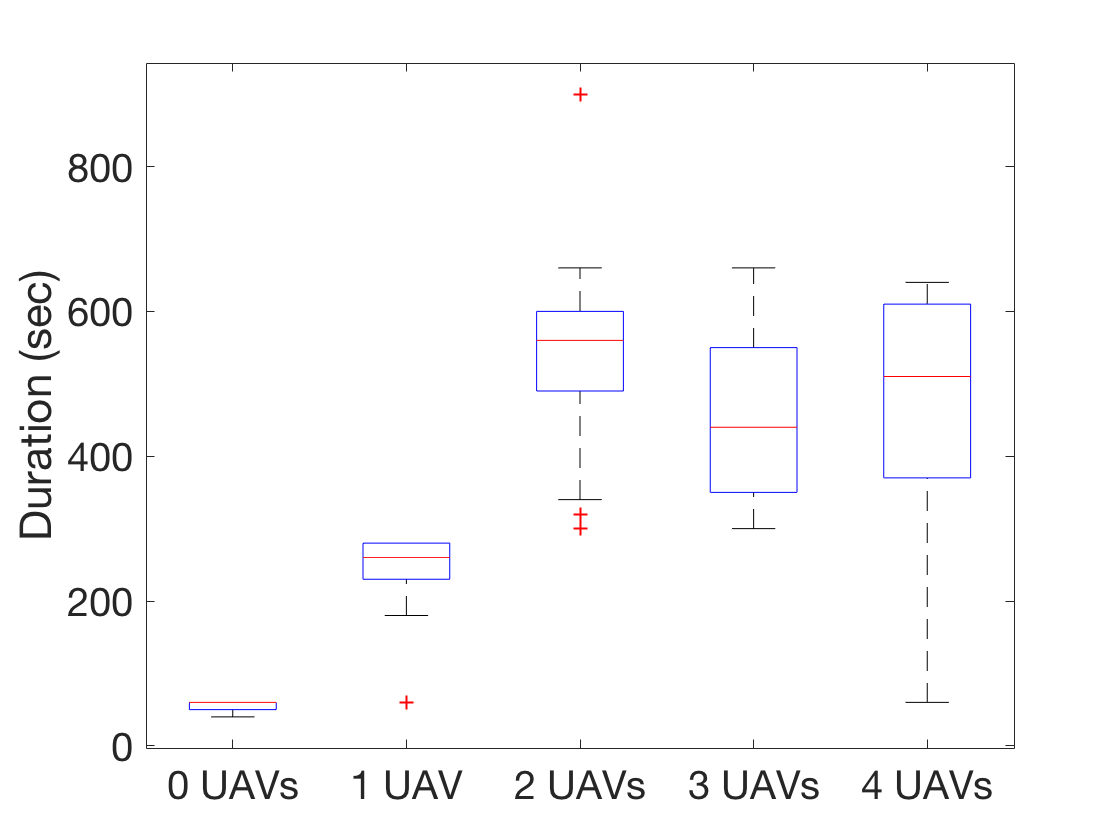
\includegraphics[width=1\linewidth]{case3_resultsgraph}
		\caption{Scenario 3}%: Mid-start with strong north wind}
		\label{fig:sub3}
	\end{subfigure}%
	\begin{subfigure}{.25\textwidth}
		\centering
		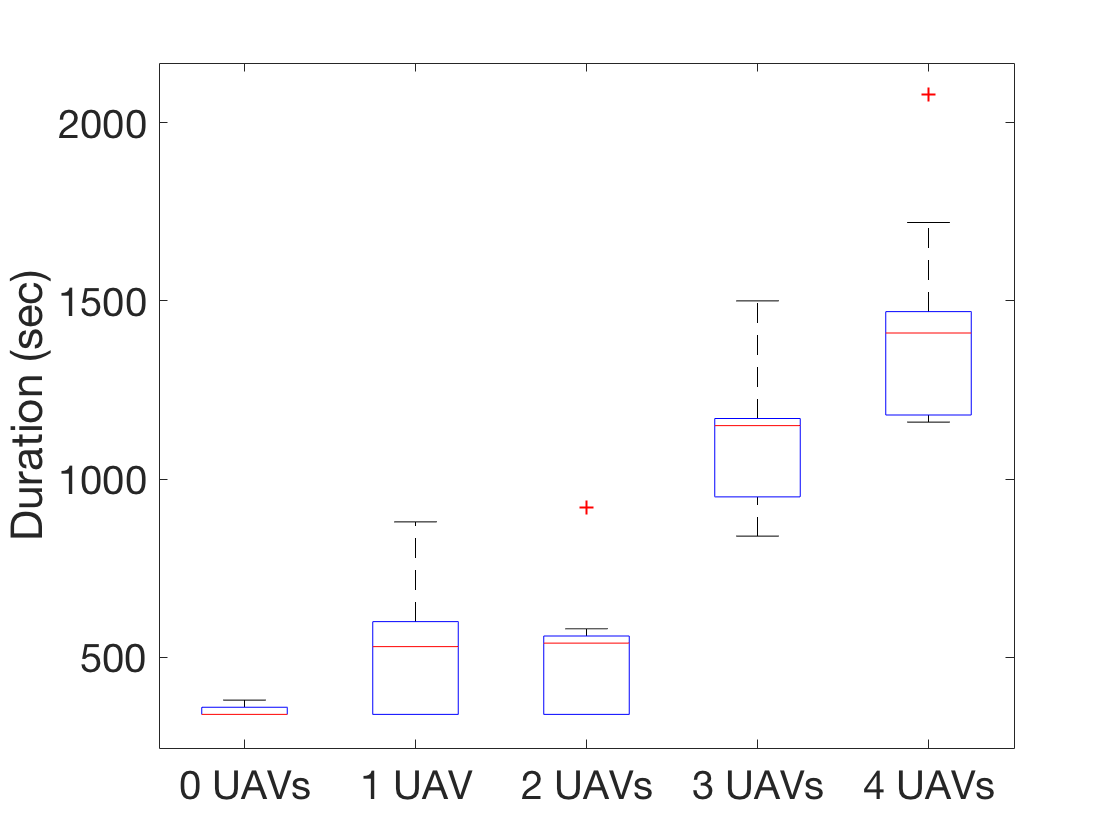
\includegraphics[width=1\linewidth]{case4_resultsgraph}
		\caption{Scenario 4}%: 2-fire base start with strong north-east wind}
		\label{fig:sub4}
	\end{subfigure}
	\caption{Distributions of simulation results for scenario 3 and scenario 4}
	\label{fig:test2}
	\vspace*{-2mm}
\end{figure}

\begin{figure}
	\centering
	\begin{subfigure}{.25\textwidth}
		\centering
		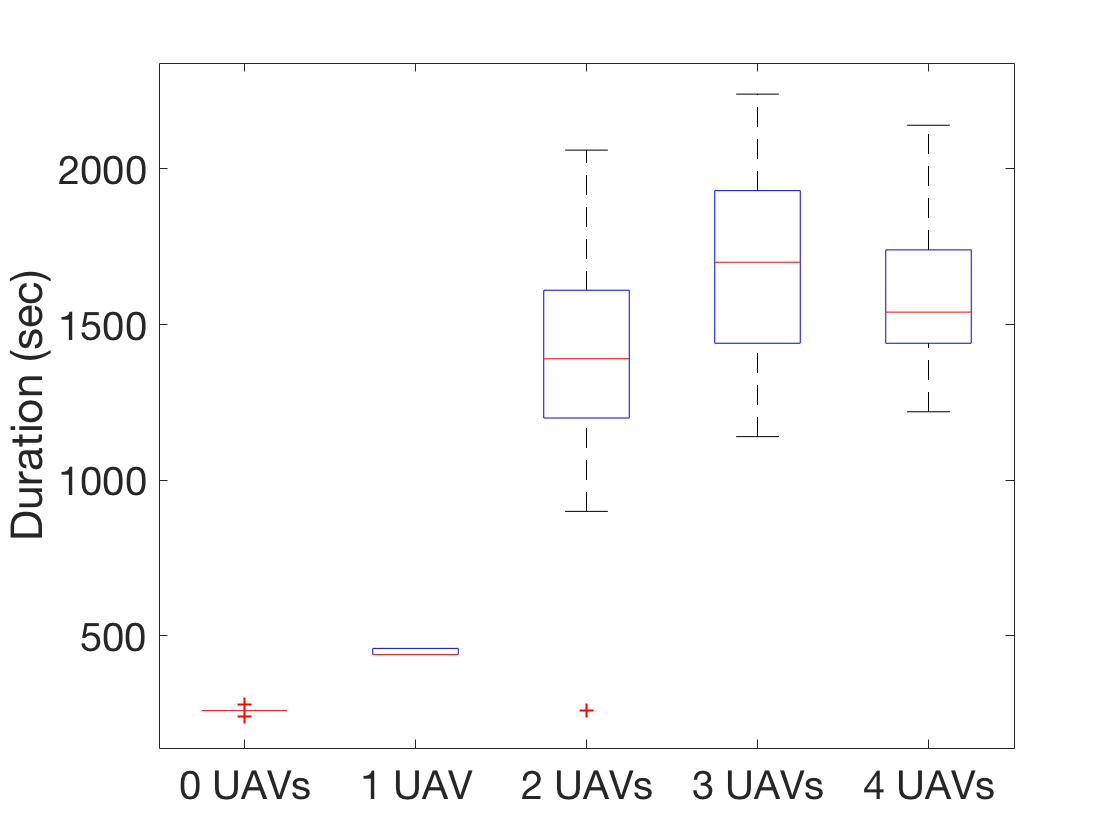
\includegraphics[width=1\linewidth]{case5_resultsgraph}
		\caption{Scenario 5}%: Low-start through choked region with medium north wind}
		\label{fig:sub5}
	\end{subfigure}%
	\begin{subfigure}{.25\textwidth}
		\centering
		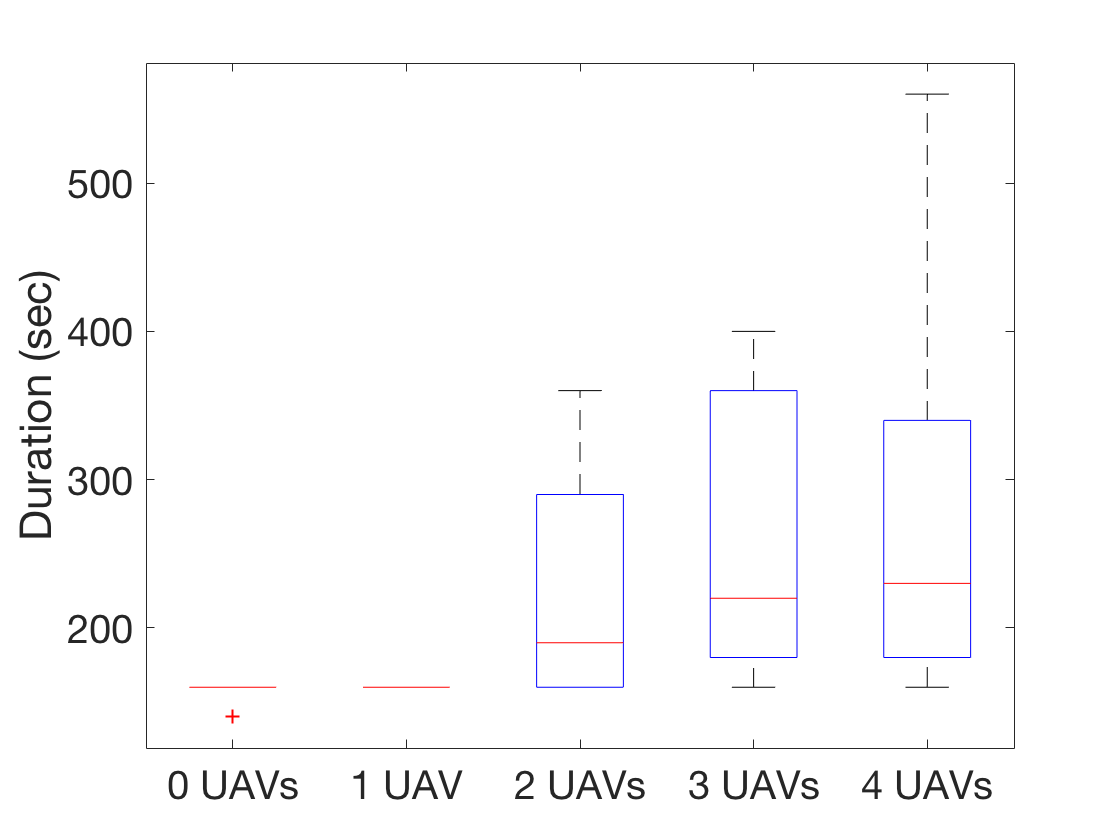
\includegraphics[width=1\linewidth]{case6_resultsgraph}
		\caption{Scenario 6}%: 2-fire high and low starts with medium east wind}
		\label{fig:sub6}
	\end{subfigure}
	\caption{Distributions of simulation results for scenario 5 and scenario 6}
	\label{fig:test3}
	\vspace*{-2mm}
\end{figure}

Table \ref{results_tab} provides an overview of the average duration times for using no UAVs in each scenario compared with the average duration times through the use of UAVs.

\begin{table}[H]
	\centering
	\caption{Average duration times for each scenario and number of UAVs used}
	\label{results_tab}
	\scalebox{0.8}{
		\begin{tabular}{|c||c||c||c||c||c|}
			\hline
			\multicolumn{1}{|p{1.2cm}|}{\centering Scenario \\ Number} & \multicolumn{1}{|p{1.2cm}|}{\centering 0 UAV (sec)} &
			\multicolumn{1}{|p{1.2cm}|}{\centering 1 UAV (sec)} & 
			\multicolumn{1}{|p{1.2cm}|}{\centering 2 UAV (sec)} & 
			\multicolumn{1}{|p{1.2cm}|}{\centering 3 UAV (sec)} & 
			\multicolumn{1}{|p{1.2cm}|}{\centering 4 UAV (sec)} \\ 
			\hline
			1 & 1024 & \multicolumn{1}{|p{1.2cm}|}{\centering 5203 \\ (+508\%)}  & \multicolumn{1}{|p{1.2cm}|}{\centering 9864 \\ (+963\%)} & \multicolumn{1}{|p{1.2cm}|}{\centering 14323 \\ (+1399\%)} & \multicolumn{1}{|p{1.2cm}|}{\centering 18881 \\ (+1843\%)} \\ 
			\hline
			2 & 159 & \multicolumn{1}{|p{1.2cm}|}{\centering 752 \\ (+percent)}  & \multicolumn{1}{|p{1.2cm}|}{\centering 1939 \\ (+percent)} & \multicolumn{1}{|p{1.2cm}|}{\centering 2033 \\ (+percent)} & \multicolumn{1}{|p{1.2cm}|}{\centering 2201 \\ (+percent)} \\ 
			\hline
			3 & 55 & \multicolumn{1}{|p{1.2cm}|}{\centering 241 \\ (+percent)}  & \multicolumn{1}{|p{1.2cm}|}{\centering 535 \\ (+percent)} & \multicolumn{1}{|p{1.2cm}|}{\centering 457 \\ (+percent)} & \multicolumn{1}{|p{1.2cm}|}{\centering 478 \\ (+percent)} \\ 
			\hline
			4 & 352 & \multicolumn{1}{|p{1.2cm}|}{\centering 495 \\ (+percent)}  & \multicolumn{1}{|p{1.2cm}|}{\centering 498 \\ (+percent)} & \multicolumn{1}{|p{1.2cm}|}{\centering 1089 \\ (+percent)} & \multicolumn{1}{|p{1.2cm}|}{\centering 1401 \\ (+percent)} \\ 
			\hline
			5 & 258 & \multicolumn{1}{|p{1.2cm}|}{\centering 449 \\ (+percent)}  & \multicolumn{1}{|p{1.2cm}|}{\centering 1331 \\ (+percent)} & \multicolumn{1}{|p{1.2cm}|}{\centering 1668 \\ (+percent)} & \multicolumn{1}{|p{1.2cm}|}{\centering 1614 \\ (+percent)} \\ 
			\hline
			6 & 159 & \multicolumn{1}{|p{1.2cm}|}{\centering 160 \\ (+percent)}  & \multicolumn{1}{|p{1.2cm}|}{\centering 220 \\ (+percent)} & \multicolumn{1}{|p{1.2cm}|}{\centering 257 \\ (+percent)} & \multicolumn{1}{|p{1.2cm}|}{\centering 274 \\ (+percent)} \\ 
			\hline
		\end{tabular}
	}
\end{table}

Additionally, example time lapses for Scenarios 1, 4, and 6 are presented in Fig. \ref{ResultsShow1}, \ref{ResultsShow2} and \ref{ResultsShow3}, showcasing how the fire grew in response to a varying number of UAVs.

\begin{figure}
	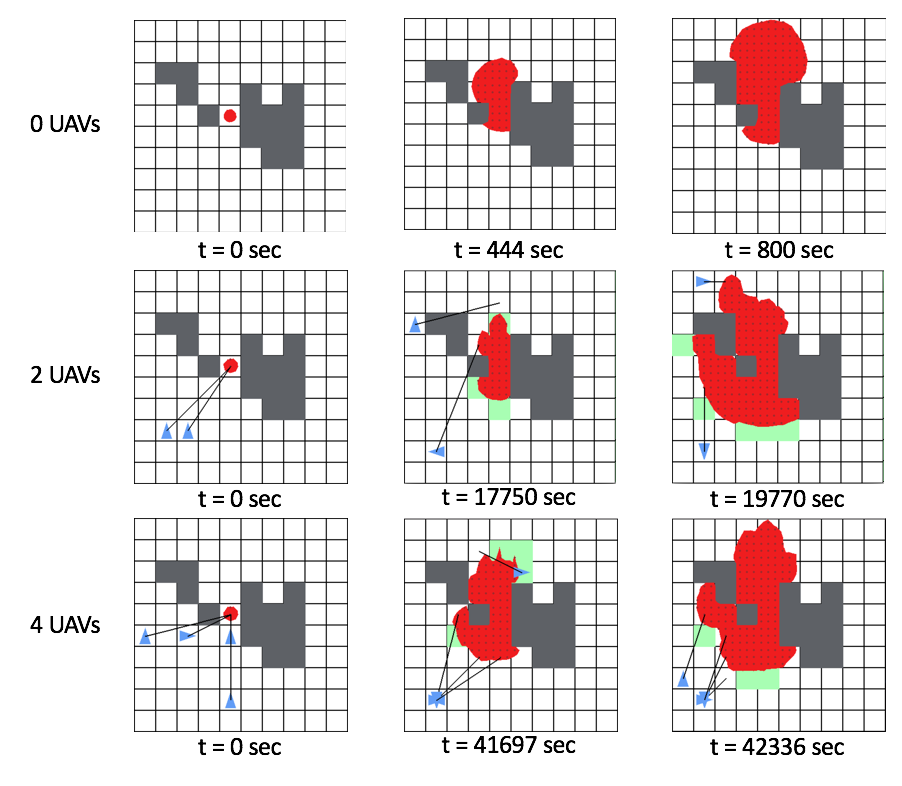
\includegraphics[width = 1 \linewidth]{case1_visuals}
	\centering
	\caption{Example of scenario 1 results for no UAVs, 2 UAVs, and 4 UAVs}
	\label{ResultsShow1}
	\vspace*{-2mm}
\end{figure}

\begin{figure}
	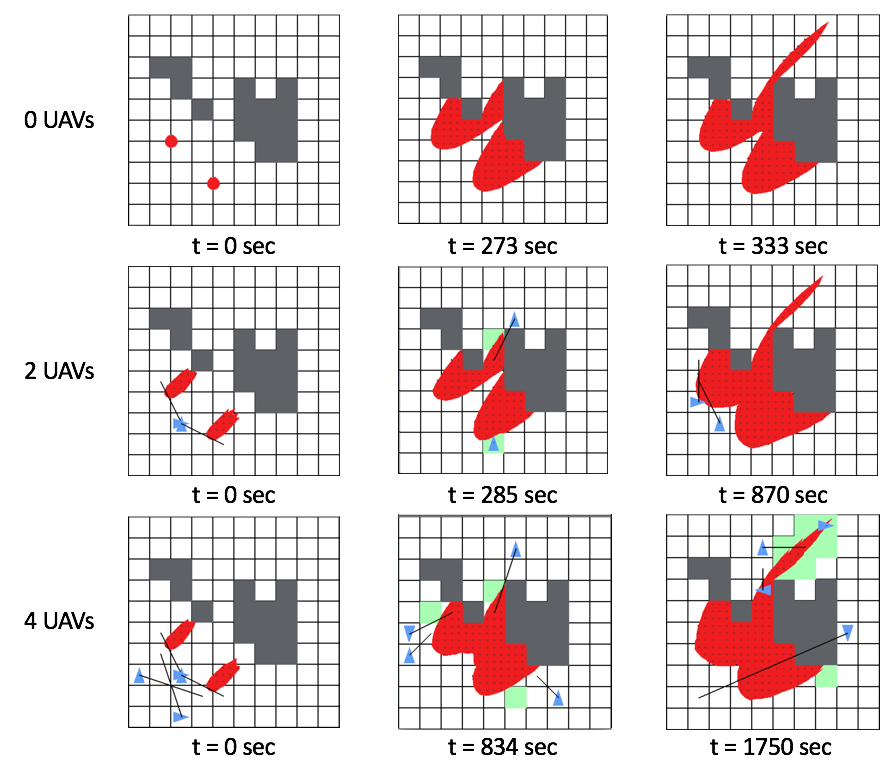
\includegraphics[width = 1 \linewidth]{case4_visuals}
	\centering
	\caption{Example of scenario 4 results for no UAVs, 2 UAVs, and 4 UAVs}
	\label{ResultsShow2}
	\vspace*{-2mm}
\end{figure}

\begin{figure}
	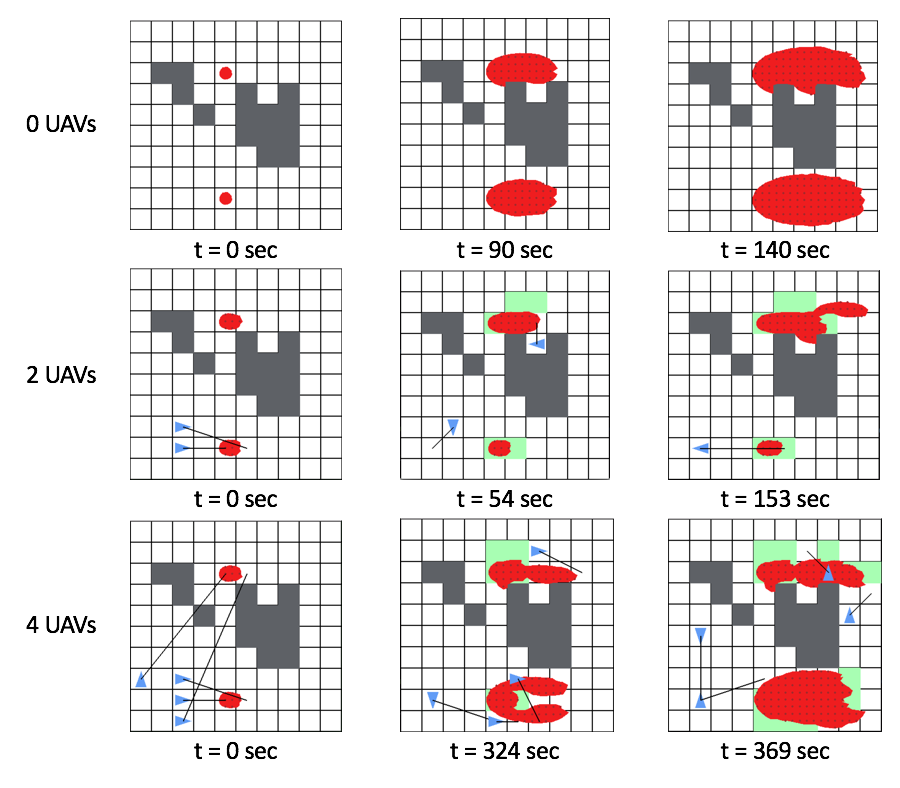
\includegraphics[width = 1 \linewidth]{case6_visuals}
	\centering
	\caption{Example of scenario 6 results for no UAVs, 2 UAVs, and 4 UAVs}
	\label{ResultsShow3}
	\vspace*{-2mm}
\end{figure}

A few outcomes are observable through Fig. \ref{fig:test}, \ref{fig:test2}, and \ref{fig:test3}. First, in all cases, increasing the number of UAVs generally increased the median and average duration times of the tests, an intuitive result. Additionally though, especially evident in Fig. \ref{fig:sub1}, the greater the amount of UAVs used resulted in a higher spread between the minimum and maximum test duration times. The most likely explanation for this behavior is that greater differences between fire conditions in separate simulations accumulate over longer run-times associated with larger UAV groups, and since the UAVs are suspect to 4 minute periods of stopping while the standard 33\% of 125 liters suppressant dropped corresponds to 3.33 minutes of burn-through time, these differences can greatly effect the UAVs' ability to slow down critical fires in time before refilling. 

The higher stress scenarios 4 and 6 (higher wind and number of fires) provide notable results in contrast to one another. In scenario 4, the obstacles provide additionally blockage for the UAVs, and as a result, a greater amount of UAVs provides greater performance since the number of critical fire locations (e.g. fires further in the wind direction and closer to the edge) are limited and easily accessible in time. This is evident in Fig. \ref{ResultsShow2} in the 300 second time of the 2 UAV case. By only hitting the edges of the fire about to wrap around the obstacle, the fire was greatly slowed down. On the other hand, in scenario 6, few obstacles slowed the fires down, and the UAVs had to ``rush" in time to suppress the fires. Multiple UAVs were always required for the test to have any chance of lasting longer than the 0 UAV case, but often UAVs could not reach the critical fires in time, evident in both the 2 UAVs and 4 UAVs cases of Fig. \ref{ResultsShow3} and by the minimum duration values in Fig. \ref{fig:sub6}.
%\vspace*{-3mm}
\section{Conclusion and Future Work}

In this paper, we constructed a high-level planner and controller to control a fleet of UAVs for various fire fighting scenarios. We simulated this method's ability to slow down the advancement of fire fronts towards the domain edge, demonstrating the potential usefulness of automated UAVs in tackling fires before crews can arrive. The ability to slow down a starting fire by even half an hour (comparable to the maximum slowdown amounts in Scenarios 1, 2 and 5) is a significant amount of time for ground crews to reach a location fast enough to effectively stop such a fire.

Expanding upon the receding horizon framework for reactive synthesis allowed us to expand the scope of this problem while integrating the method with dynamic allocation for assigning UAVs. Even with such an approach, numerous issues arose throughout the process that help highlight key difficulties moving forward when using reactive synthesis in the control of UAVs. First, the RH framework, when considering all initial conditions, still yields an excessively large controller (about 2 GB) after 8 hours of runtime, a significant hurdle for applying such a design to arbitrary obstacle environments. Next, a simplified transition system was utilized which limited the total orientation space and interpreted UAV movement in only 2 dimensions, still far more restrictive than UAV movement in reality. Lastly, no constraints were used in considering the orientation of UAVs when dropping suppressant, which significantly factors into how well the suppressant slows down an advancing fire front. Each of these points combine to exemplify the need for smarter partitioning of possible transitions a UAV can take in 3D space (easily dependent on at least 3 full degrees of freedom), should reactive synthesize be used for UAV control. So while the reactive synthesis design is strong in enforcing the design constraints formally, the scope of its application is still limited per goal.

For improvements on this problem as it was explored, multiple changes can be assessed. First, modifications to the synthesized controllers can be made to enforce desired orientations during suppressant drops. This will intuitively add to the size of the controllers but enable more accurate control of the UAVs for dropping suppressant in the correct direction. Second, direct coordination between synthesized controllers should be explored to control the frequency of suppressant drops on critical fires. The need for such is demonstrated in Fig. \ref{ResultsShow2}. If the UAVs had spread out the times they dropped suppressant on the fire wrapping around the obstacle edge, the advancement of such would be hindered further since each UAV would spend time refilling separately. This effect could be achieved through modifying the allocation algorithm to also consider assignments based on time. Lastly, the size of the synthesized controller could be addressed through reformatting the outputted synthesized controller in each horizon. Currently, controllers are synthesized per initial condition in a horizon, but synthesizing a single controller for each horizon that includes all initial conditions can cut down on the total size of the generated finite state machine.

\bibliographystyle{IEEEtran}
\bibliography{sample}

%\vspace*{-3mm}
%\begin{thebibliography}{1}
%\bibitem{c0}	
%D. Thomas, D. Butry, S. Gilbert, D. Webb, and J. Fung, ``The costs and losses of wildfires: a literature survey," \textit{Special Publication (NIST SP)}, Nov. 2017. 
%\bibitem{c1}
%D. Werner, ``Fire Drones," \textit{Aerospace America}, pp. 28–31, 2015. 
%\bibitem{c10}
%T. Wongpiromsarn, U. Topcu and R. M. Murray, ``Receding Horizon Temporal Logic Planning," \textit{IEEE Transactions on Automatic Control}, vol. 57, no. 11, pp. 2817-2830, Nov. 2012.	
%\bibitem{c2}
%H. Qin et al., ``Design and implementation of an unmanned aerial vehicle for autonomous firefighting missions," \textit{2016 12th IEEE International Conference on Control and Automation (ICCA)}, Kathmandu, pp. 62-67, 2016.
%\bibitem{c3}
%B. Johnson, F. Havlak, H. Kress-Gazit, and M. Campbell, ``Experimental Evaluation and Formal Analysis of High-Level Tasks with Dynamic Obstacle Anticipation on a Full-Sized Autonomous Vehicle," \textit{Journal of Field Robotics}, 2017.
%\bibitem{c4}
%K. W. Wong and H. Kress-Gazit, ``Need-based coordination for decentralized high-level robot control," \textit{2016 IEEE/RSJ International Conference on Intelligent Robots and Systems (IROS)}, Daejeon, pp. 2209-2216, 2016.
%\bibitem{c5}
%J. Alonso-Mora, J. A. DeCastro, V. Raman, D. Rus, and H. Kress-Gazit, ``Reactive mission and motion planning with deadlock resolution avoiding dynamic obstacles," \textit{Autonomous Robots}, 2017.
%\bibitem{c14}
%Z. Liang, X. Yang and Y. Deng, ``A partitioning-based task allocation strategy for Police Multi-Agents," \textit{ The 26th Chinese Control and Decision Conference (2014 CCDC)}, Changsha, pp. 2124-2128, 2014.
%\bibitem{c15}
%B. Mirzapour and H. S. Aghdasi, ``Modified multi-objective hybrid DE and PSO algorithms for resource allocation in forest fires," \textit{2017 7th International Conference on Computer and Knowledge Engineering (ICCKE)}, Mashhad, pp. 187-192, 2017.
%\bibitem{16}
%P. Fiorucci, F. Gaetani, R. Minciardi, R. Sacil and E. Trasforini, ``Dynamic resource allocation for forest fire risk management," \textit{Proceedings. 15th International Workshop on Database and Expert Systems Applications, 2004}, pp. 603-607, 2004.
%\bibitem{c6}
%J. Tumova and D. V. Dimarogonas, ``Multi-agent planning under local LTL specifications and event-based synchronization," \textit{Automatica}, vol. 70, pp. 239-��248, 2016.
%\bibitem{c7}
%N. Piterman, A. Pnueli, and Y. Saar, ``Synthesis of reactive (1) designs, in Verification, Model Checking, and Abstract Interpretation." Springer, pp. 364-380, 2006.
%\bibitem{c8}
%A. Ulusoy and C. Belta, ``Receding horizon temporal logic control in dynamic environments," \textit{The International Journal of Robotics Research}, vol. 33 , no. 12, pp. 1593-��1607, Jul. 2014.
%\bibitem{c9}
%X. C. Ding, M. Lazar and C. Belta, ``Receding horizon temporal logic control for finite deterministic systems," \textit{2012 American Control Conference (ACC)}, Montreal, QC, pp. 715-720, 2012.
%\bibitem{c11}
%M. P. Plucinski, A. L. Sullivan, and R. J. Hurley, ``A methodology for comparing the relative effectiveness of suppressant enhancers designed for the direct attack of wildfires," \textit{Fire Safety Journal}, vol. 87, pp. 71-��79, 2017.
%\bibitem{c18}
%Liang Yang, Juntong Qi, J. Xiao and Xia Yong, ``A literature review of UAV 3D path planning," \textit{Proceeding of the 11th World Congress on Intelligent Control and Automation}, Shenyang, pp. 2376-2381, 2014.
%\bibitem{17}
%P. Bholowalia and A. Kumar, ``EBK-Means: A Clustering Technique based on Elbow Method and K-Means in WSN," \textit{International Journal of Computer Applications}, vol. 15, no. 9, pp. 17-24, 2014.
%\bibitem{c12}
%T. Wongpiromsarn, U. Topcu, N. Ozay, H. Xu, and R. M. Murray, ``TuLip: A software toolbox for receding horizon temporal logic planning," \textit{Proc. Int. Conf. Hybrid Syst.: Computat. Control}, pp. 313-��314, 2011.
%
%
%
%\end{thebibliography}
% biography section
% 
% If you have an EPS/PDF photo (graphicx package needed) extra braces are
% needed around the contents of the optional argument to biography to prevent
% the LaTeX parser from getting confused when it sees the complicated
% \includegraphics command within an optional argument. (You could create
% your own custom macro containing the \includegraphics command to make things
% simpler here.)
%\begin{IEEEbiography}[{\includegraphics[width=1in,height=1.25in,clip,keepaspectratio]{mshell}}]{Michael Shell}
% or if you just want to reserve a space for a photo:
%\begin{IEEEbiographynophoto}{Estefany Carrillo}
%is an graduate student at the University of Maryland, College Park, in the %Department of Electrical Engineering. She received her BS degree and M.S. in %electrical engineering from University of Maryland in 2012 and 2017, respectively.  
%\end{IEEEbiographynophoto}
% if you will not have a photo at all:

% that's all folks
\end{document}


